\documentclass[letterpaper,12pt,oneside]{article}\usepackage[]{graphicx}\usepackage[]{color}
%% maxwidth is the original width if it is less than linewidth
%% otherwise use linewidth (to make sure the graphics do not exceed the margin)
\makeatletter
\def\maxwidth{ %
  \ifdim\Gin@nat@width>\linewidth
    \linewidth
  \else
    \Gin@nat@width
  \fi
}
\makeatother

\definecolor{fgcolor}{rgb}{0.345, 0.345, 0.345}
\newcommand{\hlnum}[1]{\textcolor[rgb]{0.686,0.059,0.569}{#1}}%
\newcommand{\hlstr}[1]{\textcolor[rgb]{0.192,0.494,0.8}{#1}}%
\newcommand{\hlcom}[1]{\textcolor[rgb]{0.678,0.584,0.686}{\textit{#1}}}%
\newcommand{\hlopt}[1]{\textcolor[rgb]{0,0,0}{#1}}%
\newcommand{\hlstd}[1]{\textcolor[rgb]{0.345,0.345,0.345}{#1}}%
\newcommand{\hlkwa}[1]{\textcolor[rgb]{0.161,0.373,0.58}{\textbf{#1}}}%
\newcommand{\hlkwb}[1]{\textcolor[rgb]{0.69,0.353,0.396}{#1}}%
\newcommand{\hlkwc}[1]{\textcolor[rgb]{0.333,0.667,0.333}{#1}}%
\newcommand{\hlkwd}[1]{\textcolor[rgb]{0.737,0.353,0.396}{\textbf{#1}}}%
\let\hlipl\hlkwb

\usepackage{framed}
\makeatletter
\newenvironment{kframe}{%
 \def\at@end@of@kframe{}%
 \ifinner\ifhmode%
  \def\at@end@of@kframe{\end{minipage}}%
  \begin{minipage}{\columnwidth}%
 \fi\fi%
 \def\FrameCommand##1{\hskip\@totalleftmargin \hskip-\fboxsep
 \colorbox{shadecolor}{##1}\hskip-\fboxsep
     % There is no \\@totalrightmargin, so:
     \hskip-\linewidth \hskip-\@totalleftmargin \hskip\columnwidth}%
 \MakeFramed {\advance\hsize-\width
   \@totalleftmargin\z@ \linewidth\hsize
   \@setminipage}}%
 {\par\unskip\endMakeFramed%
 \at@end@of@kframe}
\makeatother

\definecolor{shadecolor}{rgb}{.97, .97, .97}
\definecolor{messagecolor}{rgb}{0, 0, 0}
\definecolor{warningcolor}{rgb}{1, 0, 1}
\definecolor{errorcolor}{rgb}{1, 0, 0}
\newenvironment{knitrout}{}{} % an empty environment to be redefined in TeX

\usepackage{alltt}
\usepackage[paperwidth=8.5in,paperheight=11in,top=1in,bottom=1in,left=1in,right=1in]{geometry}
\usepackage{setspace}
\usepackage[colorlinks=true,allcolors=Blue]{hyperref}
\usepackage[usenames,dvipsnames]{xcolor}
\usepackage{indentfirst}
\usepackage{titlesec}
\usepackage{multirow}
\usepackage{booktabs}
\usepackage{graphicx}
\usepackage{verbatim}
\usepackage{rotating}
\usepackage{tabularx}
\usepackage{outlines}
\usepackage{lineno}
\usepackage{array}
\usepackage{times}
\usepackage{cleveref}
\usepackage{acronym}
\usepackage[position=t]{subfig}
\usepackage{paralist}
\usepackage[noae]{Sweave}
\usepackage{natbib}
\usepackage{array}
\usepackage{pdflscape}
\usepackage{bm}
\usepackage{fixltx2e}
\usepackage[inline]{showlabels}
\bibpunct{(}{)}{,}{a}{}{,}

% page margins and section title formatting
\linespread{1.5}
\setlength{\footskip}{0.5in}
\titleformat*{\section}{\Large\bf\em}
\titleformat*{\subsection}{\singlespace\large\bf}
\titleformat*{\subsubsection}{\singlespace\normalsize\bf\em}
\titlespacing{\section}{0in}{0in}{0in}
\titlespacing{\subsection}{0in}{0in}{0in}
\titlespacing{\subsubsection}{0in}{0in}{0in}

% cleveref options
\crefname{table}{Table}{Tables}
\crefname{figure}{Fig.}{Figs.}
\renewcommand{\figurename}{Fig.}

% aliased citations
\defcitealias{LehrterIR}{Lehrter et al. in review}

%acronyms
\acrodef{chla}[chl-\textit{a}]{chlorophyll \textit{a}}
\acrodef{cgem}[CGEM]{Coastal General Ecosystem Model}
\acrodef{do}[O$_2$]{dissolved oxygen}
\acrodef{dom}[DOM]{dissolved organic matter}
\acrodef{gom}[GOM]{Gulf of Mexico}
\acrodef{lcs}[LCS]{Louisiana continental shelf}
\acrodef{marb}[MARB]{Mississippi-Atchafalaya River Basin}
\acrodef{pom}[POM]{particulate organic matter}
\acrodef{zerod}[0-D]{zero-dimensional}

%for supplemental figures/tables
\newcommand{\beginsupplement}{%
        \setcounter{table}{0}
        \renewcommand{\thetable}{S\arabic{table}}%
        \setcounter{figure}{0}
        \renewcommand{\thefigure}{S\arabic{figure}}%
     }

%knitr options


% R dependencies


% get the version based on commit date


% get online bib file


\IfFileExists{upquote.sty}{\usepackage{upquote}}{}
\begin{document}

\raggedbottom
\linenumbers
\raggedright
\urlstyle{same}
\setlength{\parindent}{0.5in}
\renewcommand\refname{References \vspace{12pt}}

\begin{singlespace}
\title{{\bf {\Large Parameter sensitivity and identifiability for a biogeochemical model of hypoxia in the northern {G}ulf of {M}exico}}}
\author{
  {\bf {\normalsize Marcus W. Beck$^1$, John C. Lehrter$^2$, Lisa L. Lowe$^3$}}
  \\\\{\textit {\normalsize $^1$USEPA National Health and Environmental Effects Research Laboratory}}
  \\{\textit {\normalsize Gulf Ecology Division, 1 Sabine Island Drive, Gulf Breeze, FL 32561}}
	\\{\textit {\normalsize Phone: 850-934-2480, Fax: 850-934-2401}}
	\\{\textit {\normalsize Email: \href{mailto:beck.marcus@epa.gov}{beck.marcus@epa.gov}}}
	  \\\\{\textit {\normalsize $^2$Dauphin Island Sea Lab, University of South Alabama}}
  \\{\textit {\normalsize Dauphin Island, AL 36528}}
	\\{\textit {\normalsize Phone: 251-861-2141 ext. 7567}}
	\\{\textit {\normalsize Email: \href{mailto:jlehrter@disl.org}{jlehrter@disl.org}}}
	\\\\{\textit {\normalsize $^3$Lockheed Martin IS \& GS - Civil, supporting the USEPA}}
	\\{\textit {\normalsize Resarch Triangle Park, NC 27709}}
	\\{\textit {\normalsize Phone: 919-541-3985,}}
	\\{\textit {\normalsize Email: \href{mailto:lowe.lisa@epa.gov}{lowe.lisa@epa.gov}}}
  \vspace{1in} 
  \\ Version Date:   Mon Dec 5 14:51:33 2016 -0600
	}
\date{}
\maketitle
\end{singlespace}
\clearpage

\begin{abstract}
\noindent Bio-geo-chemical models are useful tools in environmental sciences that can guide management and policy-making. Consequently, significant time and resources are spent developing these models in system-specific contexts. The optimization of model parameters to maximize precision, including transferability of these models to different systems, are fundamental concerns in the development and application of these tools. This study provides a context for understanding quantitative limitations of coupled hydrodynamic-ecological models by evaluating parameter sensitivity and identifability of a \ac{zerod} unit of a larger spatio-temporal model of hypoxia on the \acl{lcs} of Gulf of Mexico.  The analysis provides a contrast of numeric and ecological certainty in parameter subsets using a systematic framework to infer larger trends in dissolved oxygen dynamics over time, having implications for understanding factors that contribute to environmental conditions that are detrimental to aquatic resources.  In particular, we focus on issues of parameter identifiability using local sensitivity analyses to provide quantitative descriptions of numerical constraints on model precision.  We argue that quantitative and ecological certainty in model calibration are often at odds and practitioners must choose explicit model components to optimize given tradeoffs between the two. We further conclude that numerically optimal parameter sets for models of hypoxia are often small subsets of the complete parameter set because of redundancies in the unique effects of parameter perturbations on model output.  As a result, we demonstrate that use of a model for inference into ecological mechanisms of observed or predicted changes in hypoxic condition can be potentially misguided in the absence of quantitative descriptions of identifiability.  Although these concerns have been expressed in the literature, they are rarely explicitly addressed or included in model evaluations.  In addition to immediate implications for regional models, we provide a framework for describing the effects of parameter uncertainty and identifiability that can be applied to similar models to better inform environmental management.
\end{abstract}
\acresetall

\section{Introduction}

Hypoxia formation in bottom waters of coastal oceans occurs primarily from excess nutrient inputs from land-based sources \citep{Justic87,Diaz95,Howarth96}.  These events are detrimental to aquatic organisms and have significant negative effects on economic resources derived from coastal ecosystems \citep{Lipton03,Diaz11}.  An understanding of the biological, physical, and chemical processes that contribute to the growth of hypoxic areas is a critical concern for mitigating and preventing these negative impacts.  Numerical ecosystem models are important tools that synthesize knowledge of ecosystem processes that contribute to hypoxia formation and for predicting the effects of proposed management activities or future scenarios \citep{Scavia04,Hagy07,Pauer16}.  Unlike statistical models with more generic structures, simulation and process-based models include explicit descriptions of relevant processes that are constrained by empirical or observational data relevant to the system of interest \citep[e.g.][]{Omlin01b,Eldridge10}.  These models are often coupled with hydrodynamic grids to provide spatially-explicit representations of patterns in three dimensions \citep{Warner05,Zhao10,Ganju16}. Combined hydrodynamic and bio-geo-chemical models have been developed specifically to describe hypoxic conditions on the \ac{lcs} in the northern \ac{gom} (\citealt{Fennel13,Obenour15,Pauer16}, \citetalias{LehrterIR}).  This area drains a significant portion of the continental United States through the \ac{marb} and is the second largest hypoxic area in the world \citep{Rabalais02}.  Understanding processes that contribute to the frequency and duration of hypoxic events remains a critical research goal for the region, including the application of process-based models to characterize the current knowledge domain.  

The development and application of a model represents a tradeoff between characteristics expected from the output or provided by the structural components. An idealized model is sufficiently generalizable across systems, provides results that are precise given the inputs, and includes components that are realistic descriptions of actual processes \citep{Levins66}. Given that these characteristics cannot be simultaneously achieved, models are developed in partial dependence of reality and theoretical constructs, completely separate from both, or dependent on one or the other \citep{Morrison99,Ganju16}.  These challenges are analagous to the well-known bias-variance tradeoff in statistical models that balances the competing objectives of over- and under-fitting to an observed dataset. Process-based models are more commonly imbalanced between reality and theory, such that most are over-parameterized in an attempt to completely describe reality \citep{Denman03,Nossent12,Petrucci14}.  Such over-parameterization, including use of many  structural equations, can have serious implications for practical applications.  Quantitative limitations of over-parameterization are analagous to degrees of freedom in standard statistical models as free parameters cannot be numerically estimated when constrained to an observed dataset \citep{Kirchner06}.  More importantly, over-parameterization can limit use across systems outside of the data domain and impose uncertainty in model predictions as realistic values for every variable may not be known or inaccurately applied from existing studies \citep{Durand02,Refsgaard07,Wade08}. The application of process-based models to describe hypoxia dynamics has not been immune to these challenges and comprehensive approaches are needed to develop models that more carefully balance theory with reality \citep[e.g.,][]{Snowling01}.  

Standard approaches for uncertainty analysis can be used to begin addressing model complexity issues.  In the most general sense, uncertainty is evaluated relative to the effects of input conditions or the observed data used to calibrate a model, changes in parameter values, or variation in the structural components (i.e., observational, parameter, or structural uncertainty) \citep{Beck87}.  Evaluating parameter uncertainty is by far the most common and simplest means of evaluating model behavior.  Although uncertainty analyses should be integrated throughout model development and application, parameters are more often evaluated post-hoc as a form of `damage control' for further calibration.  This approach is sometimes called inverse modelling where results from sensitivity analyses are used to guide calibration or fit of the developed model to observations (\citealt{Soetaert10}, or confronting models with data, \textit{sensu} \citealt{Hilborn97}).  Parameter sensitivity analysis combined with inverse modelling necessarily involves questions of parameter `identifiability', where only a subset of parameters can be numerically constrained to the data as compared to the entire parameter set.  Redundancies in parameter effects lead to unidentifiable models where optimal solutions may be empirically impossible (i.e., standard algorithms will not converge) or parameter values may be non-unique leading to the right answer for the wrong reason \citep{Kirchner06}. An unidentifiable parameter or parameter set has effects on model output that can be undone or compensated for by alteration of other parameters.  The concept of identifiable parameter subsets is not foreign to hypoxia or eutrophication models  \citep{Omlin01,Estrada10,Mateus15}, although there is a clear need for greater integration of these concepts in model development \citep{Fasham06}.  Moreover, the inclusion of sensitivity and identifiability analyses in model tuning will require the adoption of conservative selection rules for parameters to calibrate given the number of unique combinations of parameter subsets for most models \citep[e.g.,][]{Wagener01, Wagener01b}.  

This study describes a parameter sensitivity analysis to evaluate identifiability of parameter subsets for a bio-geo-chemical model of hypoxia for the northern \ac{gom}.  We evaluate a simple \ac{zerod} unit of a larger spatial-temporal model to explore relationships between multiple parameter sets and hypoxia dynamics on the \ac{lcs}.  Specifically, we provide empirical results to support the assumption that models are generally over-parameterized and only a finite and smaller subset of the larger parameter set can be optimized for a given research question or dataset.  We provide explicit guidance for choosing such subsets of the parameter space given constraints on identifiability as directly related to sensitivity analyses.  The objectives are to \begin{inparaenum}[1\upshape)]
\item identify the parameters that have the greatest influence on \ac{do} using local sensitivity analysis,
\item quantify the identifiability of subsets of the total parameter space based on sensitivity,
\item and provide a set of heuristics for choosing parameters based on sensitivity, identifiability, and parameter categories.
\end{inparaenum}
These principles were also applied to other state variables predicted by the model (ammonium, \ac{chla}, irradiance, nitrate, \ac{pom}, \ac{dom}, and phosphorus). A final analysis evaluated identifiability relative to structural uncertainty to provide an example of extending these methods to more complex uncertainty assessments.  Throughout, the optimum parameter set is defined as the chosen subset that represents the maximum number of identifiable parameters. `Optimum' is both a qualitative description based on a research question or management goal and a quantitative objective based on numerical optimization criteria for fitting model output to a calibration dataset.  These results can be used to refine existing models or guide application of models to novel contexts, such as downscaling or application to new environments.  We conclude with a discussion of the implications for hypoxia formation in coastal regions, including management strategies for nutrient reduction and use of mechanistic models to inform decision-making.

\section{Methods}

\subsection{Model description}

Hypoxic events, defined  as $<$2 mg L$^{-1}$ of \ac{do} ($<$ 64 mmol m$^{-3}$), occur seasonally in bottom waters in the northern \ac{gom}.  The \ac{lcs} receives high nutrient loads from the \ac{marb} that drains a significant portion of the continental United States.  Nutrient-stimulated primary production in surface waters increases biological oxygen demand in bottom waters as sinking organic matter is decomposed \citep{Bierman94,Murrell13}.  The hypoxic area averages 15,540 km$^2$ annually (1993-2015) with minimum concentrations observed from late spring to early fall.  Seasonal variation is strongly related to carbon and nutrient export from the \ac{marb} \citep{Lohrenz08,Bianchi10}, whereas hydrologic variation, currents, and wind patterns can affect vertical salinity gradients that contribute to the formation of hypoxia \citep{Wiseman97,Paerl98,Obenour15}. 

This study evaluated the core unit of a recently developed hydrodynamic and ecological model that describes horizontal and vertical transport and mixing of state variables relevant for hypoxia in the northern \ac{gom}.  The \ac{cgem} includes elements from the Navy Coastal Ocean Model \citep{Martin00} for hydrodynamics on the \ac{lcs} and a biogeochemical model with multiple plankton groups, water-column metabolism, and sediment diagenesis \citep{Eldridge10}.  The hydrodynamic component of \ac{cgem} provides a spatially-explicit description of hypoxia using an orthogonal grid with an approximate horizontal resolution of 1.9 km$^2$ and twenty equally-spaced vertical sigma layers on the shelf (depth $\leq$ 100 m, with additional hybrid layers at deeper depths).  The biogeochemical component includes equations for 36 state variables including six phytoplankton groups (with nitrogen and phosophorus quotas for each), two zooplankton groups, nitrate, ammonium, phosphate, dissolved inorganic carbon, oxygen, silica, and multiple variables for dissolved and particulate organic matter from different sources.  Atmospheric and hydrological boundary conditions described in \citet{Hodur97} and \citet{Lehrter13} are also included in \ac{cgem}.

The core unit of \ac{cgem} is FishTank, a \ac{zerod} model that implements the biogeochemical equations in \citet{Eldridge10} and does not include any form of physical transport (i.e., advection, mixing, or surface flux) nor sediment diagenesis.  Although FishTank was developed for specific application in \ac{cgem}, it can easily be applied to other hydrodynamic grids. Accordingly, the sensitivity and identifiability analyses described below are informative for both the \ac{lcs} gridded model as well as potential applications to different systems.  The FishTank model provides estimates for the 36 state variables described above using a \ac{zerod} parcel that is uniformly mixed as a closed system.  A set of initial conditions is provided on execution of the model that is based on observations of relevant variables obtained from research cruises in the northern \ac{gom} during April, June, and September of 2006 \citep[Table 1 in][]{Murrell14}. 

Results from FishTank are based on time-dependent differential equations that describe energy flow between phytoplankton and zooplankton groups as affected by nutrient uptake rates, organic matter inputs and losses, inherent optical properties, and temperature (\citealt{Penta08,Eldridge10}, see appendix in \citetalias{LehrterIR}).  A total of 108 equations are estimated at each time step to return a value for each of the 36 state variables described by the model.  In addition to the initial conditions, 251 parameter values for each of the equations are also supplied at model execution.  These parameters define relationships among fixed effects in the equations and represent ecological properties described by the model that influence hypoxia formation.  Values for each of the parameters were based on estimates from the literature, field or laboratory-based measurements, or expert knowledge in absence of the former.  As such, a sensitivity analysis of parameter values is warranted given that, for example, literature or field-based estimates may not apply under all scenarios or expert knowledge is not completely certain \citep{Refsgaard07}.

% number of parameters evaluated, total and by category


The sensitivity of \ac{do} to perturbations of all relevant parameters for the 108 equations was estimated using a five minute timestep of FishTank simulations from January 1\textsuperscript{st} to December 31\textsuperscript{st}, 2006. Irrelevant parameters were removed for several reasons; parameters were not relevant for the \ac{zerod} model (i.e., hydrodynamic parameters), were considered physical constants, or had no effect given initial conditions.  Additionally, FishTank includes six phytoplankton and two zooplankton groups to describe complexity in community structure and foodweb dynamics.  However, structural equations for each group are identical such that chosen parameter values primarily control differences between the groups, e.g., large-bodied or small-bodied plankton, slow-growing or fast-growing plankton, etc.  Initial analyses indicated that parameter sensitivity of dissolved oxygen was identical within the six phytoplankton and zooplankton groups.  To remove obvious redundancies in the model, the sensitivity analyses were conducted using only one phytoplankton and one zooplankton group.  The final parameter set that was evaluated included 51 parameters that were further grouped into one of six categories based on applicable biogeochemical components of the model: optics ($n = $ 4 parameters), organic matter (12), phytoplankton (22), temperature (2), and zooplankton (11).  A full description of the model parameters is available as an appendix in \citetalias{LehrterIR}.  

\subsection{Local sensitivity analysis}

The analysis focused on sensitivity of \ac{do} and other state variables (noted below) in the \ac{zerod} FishTank model to identify parameters that may affect spatial and temporal variation of hypoxia in the larger model.  A local sensitivity analysis was performed by evaluating the change in \ac{do} following perturbation of each parameter from its original value.  The analyses relied exclusively on concepts used in the FME package developed for the R statistical programming language \citep{Soetaert10,RDCT16}. Parameters were individually perturbed by 50\% of the original values and the model was executed to obtain an estimate of \ac{do} sensitivity.  For each perturbation, a sensitivity value $S$ was estimated for each time step $i$ given a change for parameter $j$ as:

\begin{equation} \label{sijeqn}
S_{ij} = \frac{\partial y_i}{\partial \Theta_j}\cdot\frac{w_{\Theta_j}}{w_{y_i}}
\end{equation}

\noindent where the estimate depended on the change in the predicted value for response variable $y$ divided by the change in the parameter $\Theta_j$ multiplied by the quotient of scaling factors $w$ for each.  The scaling factors, $w_{\Theta_j}$ for the parameter $\Theta_j$ and $w_{y_i}$ for response variable $y_i$, were set as the default value of the unperturbed parameter and the predicted value of $y_i$ after perturbation \citep{Soetaert10}.  The scaling ensures the estimates are unitless such that the relative magnitudes allow comparisons of model sensitivity to parameters and state variables that differ in scale.  Sensitivity values for all $j$ parameters were summarized across the time series from $i = 1$ to $n$ as $L1$:

\begin{equation} \label{l1}
L1 = \sum|S_{ij}|/n
\end{equation}

The $L1$ value for each parameter was used as the primary measure of sensitivity for the state variables. All parameters for each of the six equation categories (optics, organic matter, phytoplankton, temperature, and zooplankton) that had non-zero $L1$ (suggesting sensitivity) were retained for identifiability analysis.  

\subsection{Identifiability and selecting parameter subsets}

Identifiability of parameter subsets was estimated from the minimum eigenvector of the cross-product of a selected sensitivity matrix \citep{Brun01,Omlin01}:

\begin{equation} \label{gameq}
\gamma = \frac{1} {\sqrt{ \min \left(\rm{EV}[\mathit{\hat{S}}^\top \mathit{\hat{S}}]\right)}}
\end{equation}

\noindent where $\gamma$ ranges from one to infinity for perfectly identifiable (orthogonal) or unidentifiable (perfectly collinear) results for parameters in a sensitivity matrix $S$.  The sensitivity functions were supplied as a matrix $\hat{S}$ with rows $i$ and columns $j$ (\cref{sijeqn}) that described deviations of predicted \ac{do} from the default parameter values.  Thus, $\gamma$ can be estimated for any subset of parameter combinations using the change in model output for perturbations of individual parameters. Sensitivity matrices were first normalized by dividing by the square root of the summed residuals \citep{Omlin01,Soetaert10}. 

The collinearity index $\gamma$ provides a measure of the linear dependence between sensitivity functions (i.e., $S_i$ for $j$ parameters) described above for subsets of parameters. Estimates of $\gamma$ greater than 10-15 suggest parameter sets are poorly identifiable \citep{Brun01,Omlin01}, meaning parameter values that maximize precision on a calibration dataset are inestimable by conventional optimization algorithms given similar effects of the selected parameters on the estimated state variable. Greater sensitivity of a state variable to a subset of parameters does not always imply better identifiability if the effects of individual parameters are similar.  An intuitive interpretation of $\gamma$ is provided by \citet{Brun01} such that a change in a state variable caused by a change in one parameter can be offset by the fraction $1 - 1/\gamma$ by the remaining parameters.  That is, $\gamma = 10$ suggests the relative change in \ac{do} for an arbitrary parameter in the selected set can be compensated for by 90\% with changes in the other parameters. 

Initial analyses suggested that considerably limited subsets of parameters were identifiable of the 51 evaluated for the FishTank model.  Given this limitation, parameter selection must consider the competing objectives of increased precision with parameter inclusion and reduced identifability as it relates to optimization.  An additional challenge is the excessively high number of combinations of parameter sets, which complicates selection given sensitivity differences and desired ecological categories of each parameter (e.g., practitioners may only be interested in optics parameters).  For example, \cref{fig:combnex} provides a simple graphic of the unique number of combinations that are possible for different subsets of `complete' parameter sets of different sizes (i.e., based on $n$ choose $k$ combinations equal to $n!/\left(k!\left(n-k\right)!\right)$).  The number of unique combinations increases with the total parameters in the set and is also maximized for moderate selections (e.g., selecting half the total).  For example, over 10$^{14}$ combinations are possible by selecting 25 parameters from a set of 50.  Accordingly, parameter selection is complicated by differing sensitivity, identifiability limits for parameter subsets, and the difficulty of choosing from many combinations.

A set of heuristics was developed that address the tradeoff in model complexity and identifiability given the challenges described above \citep[see also][]{Wagener01}.  These rulesets were developed with the assumption that parameters will be selected with preference for those with high sensitivity and identifability based on $\gamma < 15$ as an acceptable threshold for subsets (e.g., 93\% accountability).  Selection heurestics also recognized that parameter categories (i.e., optics, organic matter, phytoplankton, temperature, zooplankton) may have unequal preferences by model users given questions of interest.  In all selection scenarios, parameters were selected by decreasing sensitivity starting with the most sensitive until identifiability did not exceed $\gamma = 15$ where selections were \begin{inparaenum}[1\upshape)]
\item blocked within parameter category,
\item independent of parameter category,
\item or considering all categories equally.
\end{inparaenum} The selection rules produced seven subsets of parameters that could further be used to optimize model calibration.

\subsection{Observational and structural uncertainty}

In addition to parameter uncertainty, the effects of observational and structural uncertainty on the sensitivity analyses were evaluated by changing the initial conditions and structural components, respectively, from the default model setup.  First, observational uncertainty (i.e., effects of observed data on model output) was evaluated by varying the initial conditions that were based on observational data from research cruises in the northern \ac{gom} \citep{Murrell14}. Uncertainty in these data translates directly to uncertainty that can influence results of the sensitivity analysis.  For example, the sensitivity of \ac{do} to variation in the half-saturation constants for phytoplankton (the concentration supporting half the maximum uptake rate of nutrients) will vary given the initial nutrient concentrations \citep{Eppley69}.  Further, changes in the ratio between nitrogen and phosphorus could affect sensitivity depending on the limiting nutrient.  Parameter sensitivity was re-evaluated by varying all initial conditions that were non-zero by different seasonal means based on averages of water quality data across stations and years.  April and September seasonal averages of the observed data were used to evaluate the effects of conditions that were typical of spring and late summer on the \ac{lcs} (\cref{tab:inits}).  

The effects of model structure on parameter sensitivity (i.e., structural uncertainty) were evaluated by changing specific components of the model.  The FishTank model includes several ecosystem processes or characteristics that can be included based on expected conditions, available data, or desired complexity.  These `switches' are conceptually different from model parameters as they allow the inclusion or exclusion of explicit equations or processes.  Switches in FishTank include different structural equations for the vertical attenuation of light through the water column (inherent or apparent optical properties, \citealt{Penta09,Eldridge10}) and chlorophyll to carbon ratio models (fixed or dynamic given light and nutrients, \citealt{Cloern95}).  Several switches also affect phytoplankton growth including different models for specific growth and effects of temperature, light dependence, nutrient uptake, and internal cell quotas \citepalias[][references therein]{LehrterIR}.  

Parameter sensitivity was evaluated by comparing the results from the default model setup to a more complex setup with alternative switches (\cref{tab:strcs}).  The scenarios used switches for different equations to represent structural relationships of phytoplankton growth patterns with temperature, nutrient uptake, cell quotas, \ac{chla} to carbon ratios, photosynthesis dynamics, and specific growth limits. The default scenario modelled phytoplankton growth with temperature as a sigmoidal function \citep{Eldridge10}, nutrient uptake as Michaelis-Menten kinetics \citep{Dugdale67}, internal cell quotas following \citet{Droop73}, \ac{chla} to carbon ratios as a simple regression \citep{Murrell14}, light-dependence of photosynthesis with photoinhibition \citep{Platt80}, and a specific growth rate following Leibig's law of the minimum.  Conversely, the complex scenario used switches that modelled relationships between phytoplankton growth with temperature using the Arrhenius model \citep{Geider97}, nutrient uptake as proposed by \citet{Lehman75} and modified in \citet{Geider98}, internal cell quotas following \citet{Flynn03}, \ac{chla} to carbon ratios following \citet{Cloern95}, light-dependence of photosynthesis that is nutrient dependent \citep{Flynn03}, and a specific growth rate that is nutrient dependent.  Complete details of model switches are provided as supplementary material to \citetalias{LehrterIR}.

\subsection{Extension to other state variables}

The above analyses were repeated for additional state variables estimated by FishTank to provide further descriptions of ecological dynamics that are relevant for hypoxia.  In addition to \ac{do}, other state variables that were evaluated were ammonium, \ac{chla}, irradiance, nitrate, \ac{pom}, \ac{dom}, and phosphorus.  Particulate and dissolved organic matter were estimated as the summation of the respective outputs for organic matter from phytoplankon (\textit{OM1\_A}, \textit{OM2\_A}) and fecal pellets from zooplankton (\textit{OM1\_Z}, \textit{OM2\_Z}, see \citetalias{LehrterIR}). 

\section{Results}

% for inline

 
\subsection{Local sensitivity analysis}

Local sensitivity analyses showed that \ac{do} was sensitive to perturbations in 38 of the 51 (75\% of total) evaluated parameters in FishTank (default panel \cref{fig:sensalltile}, \cref{tab:dosens}). Within each parameter category, \ac{do} was sensitive to three parameters for optics (75\% of all optic parameters), eight for organic matter (67\%), 16 for phytoplankton (73\%), one for temperature (50\%), and 10 for zooplankton (91\%). Although \ac{do} had the greatest sensitivity to parameters in the zooplankton category (as percentage of total), the relative effects varied. Among all parameters, sensitivity values ranged from $L1 = $ $8.34\times 10^{-8}$ for \textit{QminP} (phytoplankton) to $0.05$ for \textit{umax} (phytoplankton), whereas average sensitivity among all parameters was $L1 = $ $0.01$. Within categories (excluding temperature), sensitivity ranged from $4.39\times 10^{-5}$ (\textit{astarOMA}) to $7.51\times 10^{-4}$ (\textit{astar490}) for optics, $4.17\times 10^{-4}$ (\textit{KNH4}) to $0.01$ (\textit{KG1}) for organic matter, $8.34\times 10^{-8}$ (\textit{QminP}) to $0.05$ (\textit{umax}) for phytoplankton, and $3.69\times 10^{-5}$ (\textit{ZQp}) to $0.05$ (\textit{ZKa}) for zooplankton (\cref{tab:dosens}).  Average sensitivity values in each category were $L1 = $ $2.81\times 10^{-4}$ for optics, $0$ for organic matter, $0.02$ for temperature, $0.01$ for phytoplankton, and $0.01$ for zooplankton.



Local sensitivity analyses for the additional state variables (ammonium, \ac{chla}, irradiance, nitrate, \ac{pom}, \ac{dom}, and phosphorus) had similar results as \ac{do} with some exceptions (\cref{fig:sensalltile,tab:nh4sens,tab:chlsens,tab:irrsens,tab:no3sens,tab:om1sens,tab:om2sens,tab:po4sens}).  All variables were sensitive to the same parameters as \ac{do} (38 of 51 evaluated), although average sensitivity differed between variables.  Average $L1$ ranged from $0.02$ for irradiance (\cref{tab:irrsens}) to $0.71$ for \ac{dom} (\cref{tab:om2sens}).  All average sensitivity values for the state variables were higher than the average for \ac{do} ($L1$ = $0.01$).  For each variable, $L1$ ranged from $2.24\times 10^{-6}$ (\textit{QminP}) to $8.49$ (\textit{mA}) for ammonium (\cref{tab:nh4sens}), $1.38\times 10^{-6}$ (\textit{QminP}) to $13.94$ (\textit{mA}) for \ac{chla} (\cref{tab:chlsens}), $1.92\times 10^{-7}$ (\textit{QminP}) to $0.13$ (\textit{ZKa}) for irradiance (\cref{tab:irrsens}), $6.67\times 10^{-7}$ (\textit{QminP}) to $8.49$ (\textit{umax}) for nitrate (\cref{tab:no3sens}), $6.41\times 10^{-5}$ (\textit{KNH4}) to $7.22$ (\textit{mA}) for \ac{pom} (\cref{tab:om1sens}),  $7.41\times 10^{-5}$ (\textit{KNH4}) to $14.25$ (\textit{mA}) for \ac{dom} (\cref{tab:om2sens}), and $8.21\times 10^{-7}$ (\textit{QminP}) to $1.47$ (\textit{ZKa}) for phosphate (\cref{tab:po4sens}).  For the parameter categories, ammonium was most sensitive to phytoplankton parameters (average $L1$ = $0.8$ across all parameters in the category), \ac{chla} to phytoplankton ($L1$ = $1.14$), irradiance to zooplankton ($L1$ = $0.03$), nitrate to zooplankton ($L1$ = $1.06$), \ac{pom} to temperature ($L1$ = $0.86$), \ac{dom} to temperature ($L1$ = $1.48$), and phosphate to zooplankton ($L1$ = $0.31$).  Finally, average sensitivity between parameter categories independent of the state variables ranged from $0.01$ for optics (average $L1$ across all variables) to $0.62$ for phytoplankton. 

\subsection{Subset identifiability}



The identifiability analyses suggested that many parameter subsets exceeded the thresholds of $\gamma = 10, 15$, providing further justification for using selection heuristics for parameter optimization.  Results for \ac{do} are provided first to demonstrate general concepts for the identifiability analyses, followed by an extension to the remaining state variables.  Parameter identifiability (as $\gamma$) for \ac{do} increased at different rates with increasing size of parameter subsets depending on the parameter category or the number of top parameters that were selected (\cref{fig:identplo}). By category, identifiability was lowest for all combinations of parameter subsets in the phytoplankton ($60$\% of subsets less than $\gamma = 15$, $43$\% less than $\gamma = 10$) and zooplankton categories ($53.1$\% less than $\gamma = 15$, $40$\% less than $\gamma = 10$), whereas all combinations were identifiable for optics ($100$\% less than $\gamma = 15$, $100$\% less than $\gamma = 10$) and a majority identifiable for organic matter ($91.9$\% less than $\gamma = 15$, $76.5$\% less than $\gamma = 10$). Identifiability for parameters in the temperature category was not evaluated because \ac{do} was sensitive to only one parameter (i.e., $\gamma = 1$). Parameter combinations for choosing from the top, top two, top three, and top four parameters in each category together had decreasing identifability with the increasing size of the selection pool (e.g., top one versus top four parameters, \cref{fig:identplo}).  The percentage of parameter subsets that were below the acceptable thresholds for identifability was $100$\% less than $\gamma = 15$ and $100$\% less than $\gamma = 10$ for the top parameters in each category, $90.6$\% and $80.7$\% for the top two, $80.7$\% and $70.9$\% for the top three, and $55.8$\% and $45.7$\% for the fop four.  Results for the remaining state variables had similar patterns in identifiability with increasing size of parameter subsets and selection categories, although differences in identifiabiltiy between state variables was observed (\cref{fig:identploall}).  Most notably, nitrate was consistently the least identifiable variable for all selection heuristics (highest $\gamma$), whereas \ac{do} was most identifiable.

An alternative view of the results in \cref{fig:identplo} can be used to demonstrate the effects of parameter selection criteria and number of parameters in the selection pool on identifiability.  \Cref{fig:percthresh} shows the percentage of identifiable parameter sets for \ac{do} using the same selection criteria in \cref{fig:identplo}, i.e., selection of parameters only within parameter categories and selection of the top sensitive parameters regardless of category.  \Cref{fig:percthresh} is conceptually similar to \cref{fig:identplo}, with the added effect of a chosen $\gamma$ threshold on identifability.  Previous studies have provided general rules for $\gamma$ thresholds \citep{Brun01,Omlin01}, such that exact values beyond which model calibration fails could vary for the given model and optimization method.  The selected $\gamma$ thresholds are somewhat arbitrary, although the results show differences that have implications for parameter selection for model calibration.  In general, identifiability decreased with the addition of parameters, although the rate of decrease depended on the selected threshold for $\gamma$. More conservative values for $\gamma$ (e.g., $\gamma = 5$) were more sensitive to the number of parameters in a subset, that is, identifiability decreased more quickly with the addition of parameters at lower $\gamma$ thresholds as compared to higher $\gamma$.  Notable differences in identifiability were also observed by selection criteria (within categories or top parameters only), which further supports results in \cref{fig:identplo,fig:identploall}.    



An evaluation of the effects of individual parameters on $\gamma$ suggested that some parameters had disproportionate effects on identifiability.  Based on $\gamma = 15$, \cref{fig:identplo} suggests that most parameter sets for organic matter were identifiable, regardless of how many parameters were selected (i.e., two through eight).  However, some subsets were not identifiable such that identification of one or more redundant parameters that are inflating $\gamma$ values could provide useful information.  \Cref{fig:exclex} shows an alternative view of identifiability of \ac{do} with exclusion and inclusion of individual parameters in different sets for the organic matter category.  As before, collinearity increases with more parameters in a subset, although the increase varies depending on which parameter was included or excluded from the set.  For example, inclusion of \textit{KNO3} in a parameter set almost always inflated $\gamma$.  All parameter subsets that did not include \textit{KNO3} were well below $\gamma = 15$, suggesting that removal of this parameter improves identifiability.  Interestingly, the inclusion of some parameters caused a reduction in $\gamma$, which contradicts the general rule that more parameters caused reduced identifiablity.  For example, parameter sets that included \textit{KGcdom} generally had lower $\gamma$ values relative to those that excluded the parameter.

\subsection{Parameter selection}



The above results demonstrated that the state variables differed in the magnitudes of sensitivity for each parameter and the number of identifiable subsets, where the latter varied by identifiability thresholds and parameter selection criteria.  These results further underscore the need for explicit selection heuristics for parameters to calibrate for improving model performance. Results for each of the three selection heuristics (blocked by parameter category, independent of category, all categories equally) applied to each state variable differed in the number of selected parameters and distribution of parameters within each category (\cref{tab:heurist1,tab:heurist2,tab:heurist3}).  In general, a corresponendence was observed between the number of parameters that were selected given the threhold of $\gamma = 15$ and relative identifiability between the state variables.  As noted above, nitrate was the least identifiable variable (\cref{fig:identploall}), whereas other variables (e.g., \ac{do}, irradiance) were more identifiable.  The constraints on relative identifiability between variables were demonstrated with the selection heuristics.  For example, heuristics for nitrate typically selected only one or two parameters that met the criteria as compared to more identifiable variables that included several parameters that were identifiable. Overall, the first selection heuristic demonstrated that the number of parameters chosen by parameter category differed independently of the state variables (\cref{tab:heurist1}). The number of selected parameters averaged across state variables in decreasing order was 4.25 parameters from the phytoplankton category, 3.5 from organic matter, 2.75 from optics, and 2.38 from zooplankton.  These rankings were independent of parameter sensitivity and identifiability in each category.  The second and third selection heuristics (\cref{tab:heurist2,tab:heurist3}) were similar, although more parameters were generally selected for the third heuristic.

\Cref{fig:heurist_stts} demonstrates parameter selection for all state variables following the second heuristic where parameters were chosen by decreasing sensitivity independent of parameter categories (exact values are shown in \cref{tab:heurist2}).  The y-axis on the plot shows the relative identifiability values with the addition of parameters from one to many on the x-axis (from left to right).  The second to last parameter for each variable is the last parameter selected within the potential threshold of $\gamma = 15$.  Interestingly, the last parameter shown for most of the state variables caused a relatively large increase in $\gamma$ that was disproportionate to the combined identifiability of the preceding parameter set. For most variables, the phytoplankton edibility vector for zooplankton (\textit{ediblevector(Z1)}) caused a dramatic increase in $\gamma$ with inclusion in the parameter set.  In addition to demonstrating the approach for selection with the second heuristic, \cref{fig:heurist_stts} provides an alternative method of identifying parameters that are disporportionately redundant within a given parameter set.  This infomation is useful if additional parameter selection rules are developed independently of those proposed herein. 

\subsection{Observational and structural uncertainty}

Both the relative $L1$ estimates and number of parameters that affected state variables were sensitive to variation in the initial conditions (observation effects) and structural changes in the model.  Visual comparison of sensitivity values ($L1$) for the default model setup showed that all state variables were sensitive to \textit{vmaxSi} after changing the initial conditions to April or September conditions (\cref{fig:sensalltile}).  State variables were also sensitive to \textit{Ksi} for only the September conditions. Changing the model structure from the default (simple) to the complex setup showed state variables were also sensitive to \textit{KQn} and \textit{Tref(nospA+nospZ)$_{z1}$}.  Changes in the sensitivity of individual parameters were also observed, most notably as a disproportionate increase in $L1$ for ammonium, \ac{chla}, \ac{pom}, and \ac{dom} to \textit{mA} and \textit{Tref(nospA+nospZ)$_{p1}$} using the complex model setup.  Summaries by parameter categories of the effects of initial conditions and structural changes are shown in \cref{tab:inistrchg,fig:inistrsumm}. Changes in average sensitivity using April and September initial conditions showed most variables were less sensitive to parameters in the optics, temperature, and zooplankton categories, whereas increased sensitivity was generally observed for parameters in the organic matter and phytoplankton categories.  Some exceptions were observed, such as a decrease in nitrogen sensitivity to phytoplankton parameters.  Effects of structural complexity were most apparent as an increase in sensitivity of state variables to phytoplankton and temperature parameters, as noted for the individual variables in \cref{fig:sensalltile}. 

\section{Discussion}

\subsection{Implications of sensitivity and identifiability analyses}

Common goals in the application of biogeochemical models of ecosystem processes are to \begin{inparaenum}[1\upshape)]
\item accurately describe the system my matching predictions with observed data \citep{Reckhow90}, and 
\item provide a means of forecasting ecosystem condition with hypothesized management or environmental scenarios \citep{Clark01}. 
\end{inparaenum}
Although these objectives are the focus of most model applications, the structural components of process-based models should secondarily provide inference into which ecosystem processes and functions are driving observed or hypothesized changes.  This latter objective represents a more general scientific outcome of biogeochemical models that extends beyond the applied benefits of describing and predicting change in a particular system.  Modelers often hope to identify universal principles that govern dynamics across systems and the constraint of model parameters to observations provides a means of supporting or refuting hypotheses \citep{Kirchner06}.  Extension of these principles to test the effects of structural changes and observation uncertainty on model predictions provides further evidence to validate model components. This study provided a simple approach to use the effects of parameter perturbations on model state variables to characterize identifiable parameter subsets that vary by parameter selection criteria.  By doing so, we demonstrated that small parameter subsets relative to all sensitive parameters were within the identifiabilty thresholds described in the literature.  The identifiable parameter subsets varied considerably between state variables and the method for parameter selection.  We further demonstrated that changes in the model structure and variation in the initial conditions had an effect on sensitivity which has direct implications for identifiability. In general, these results provide justification for the use of explicit parameter selection heuristics that practitioners should adopt for model calibration.

Although the results were specific to individual variables, some generalities can be inferred from the sensitivity analyses. State variables were most sensitive to parameters in the phytoplankton and zooplankton categories, particularly the maximum growth rates (\textit{umax} for phytoplankton, \textit{Zumax} for zooplankton), mortality coefficient for phytoplankton (\textit{mA}), and the zooplankton half saturation coefficent for grazing (\textit{ZKa}). An increase in growth rate of primary producers has the potential to increase oxygen concentration through photosynthetic processes, although increased production of organic matter is balanced with respiration and bacterial decomposition that reduce \ac{do} concentration in the water column.  Similarly, increases in zooplankton abundance with increased growth rates causes a reduction in phytoplankton biomass through grazing, which is expected to further deplete pools of organic matter.  Most variables were also sensitive to variation in the half-saturation grazing coefficient which moderates the concentration of nutrients that support half the maximum grazing rate. Although the tradeoff between abundance, grazing, and decomposition is complex, the sensitivity of model state variables to parameters that directly control the abundance of primary producers is in agreement with empirical observations of factors that influence hypoxia dynamics on the \ac{lcs} \citep{Fahnenstiel95,Roelke00,Eldridge10}. The sensitivity of the model output to variation in other parameters that relate to physical and chemical properties of the system was of secondary importance to biological relationships.  State variables were sensitive to changes in light and temperature parameters, although to a lesser extent than phytoplankton and zooplankton parameters.  As such, the differing sensitivities of state variables to parameters in each of the categories was not unexpected given general ecological relationships that are well understood and described by the model.    

The overwhelming conclusion from the identifiablity analyses is that only limited subsets of parameters are identifiable within the constraints of local sensitivity analyses. Although we have not attempted actual model calibration (see recommendations below), these results support previous studies that have suggested similarly small subsets of parameters can be identified using traditional calibration schemes \citep[e.g.,][]{Wheater86,Ye97,Omlin01}.  In addition to \ac{cgem}, these conclusions have relevance for many biogeochemical models that include numerous parameters and structural equations to characterize processes in the model domain.  A general conclusion is that perhaps a trend towards less complex models could be beneficial given that only a small subset of parameters is identifiable and that ecosystem processes may in fact be sufficiently characterized with few parameters \citep{Ye97}.  Conversely, others have argued that model complexity is not in itself a disadvantage when parsimony is not the sole arbitrator of model structure \citep{Reichert97}. Over-parameterization can be useful if processes have importance that were not evaluated during model identification.  Single objective functions that maximize model precision with identifiable parameters may also provide an incomplete characterization of model worth, which has prompted the development of probability-based models of hypoxia that explicitly include uncertainty in model components \citep[e.g.][]{Obenour15}.  Our results demonstrated that approximately 75\% of the evaluated parameters had an effect on the eight state variables, whereas \ac{cgem} includes a total of 36 variables and multiple plankton groups, not all of which have immediate concern for understanding hypoxia. The redundancies identified with the sensitivity analyses are only problematic if the primary interest is, for example, \ac{do} dynamics.  Moreover, the proposed parameter selection heuristics provide flexibility for selecting different parameters based on parameter categories with the assumption that the chosen parameters depends on the research or management question. 

Results from the identifiability analyses provided additional insight into the interactions of parameters in large biogeochemical models.  First, identifiability of parameter subsets was not related to the sensitivity of individual variables. As noted above, an identifiable parameter is one that has a unique effect on model predictions that cannot be compensated for or undone by changing values of other parameters. The magnitude of the effect has no bearing on identifiability, which further complicates the selection of parameters for calibration.  Although identifiability is the primary limiting factor in choosing a given set, the relative sensitivities are more important for the decision to include or exclude indvidual parameters.  Our analysis addressed this challenge by presenting multiple selection criteria for identifiable parameter sets that prioritized the most sensitive parameters during the selection process.  Similarly, identifability was not always related to the number of parameters in a set. Although the overwhelming trend was decreasing identifiability with more parameters, the unique effects of including an individual parameter with an existing set often reduced the $\gamma$ estimate. For example, \cref{fig:exclex} shows that including \textit{KGcdom}, \textit{KO2}, or \textit{nitmax} in parameters sets more often reduced $\gamma$ relative to sets that excluded the parameters.  Conversely, \cref{fig:heurist_stts} showed that the inclusion of a specific parame ters often caused a disporportionate increase in $\gamma$ (e.g., \textit{ediblevector(Z1)}). These examples demonstrate the complex interactions of parameter changes on variable response, highlighting the need to consider the combined and individual effects of parameters on identifiability. The selection criteria proposed in our above analyses can facilitate parameter selection and also provide diagnostic tools to identify parameters with disproportionate effects on $\gamma$.

\subsection{Recommendations and conclusions}

An evaluation of parameter uncertainty and identifiability of relevant parameter sets is a preliminary and simplistic approach to improving model predictions.  In general, uncertainty analyses that lead to improved models are ultimately expected to increase our understanding of properties that define ecosystems using relationships described by the model.  The extension of simple parameter sensitivity analyses to the generalization of ecosystem properties requires additional analysis and potential model refinement, at the core of which is the balance between generality and precision. We emphasize that the utility of a specific model depends on the question and objective for application to a specific system.  For the above analysis, the FishTank model as part of the larger \ac{cgem} application was evaluated in the context of hypoxia effects on ecosystem condition and function.  At the core of the simple model is a set of biogeochemical equations that characterize the system in relation to planktonic groups, nutrient requirements, and water-column metabolism.  Our results have shown that relatively small subsets of parameters are identifiable given the complexity of the model, and as a result, we have provided a general approach to select parameter subsets depending on the ecological context (i.e., selection by parameter category, selection for specific state variables).  Thus, the results described above have relevance for further model refinement with the specific goal of better understanding ecological dynamics that moderate hypoxia on the northern \ac{gom}.  However, the general principles of sensitivity and parameter identifiability have broad applicability beyond this context and we argue that such methods should be more universally applied as an initial approach to quantify numerical constraints of biogeochemical models.  

Specific approaches can be used to improve and build on the results presented herein, in addition to the more general considerations noted above. A logical next step is an evaluation of model precision following calibration with relevant parameter subsets.  For simplicity, our analysis did not calibrate model parameters and an explicit assumption was that parameter subsets with $\gamma$ below 10 or 15 were identifiable.  To our knowledge, this threshold has not been rigorously evaluated and a logical expectation is that this threshold is likely to vary between parameter subsets and the chosen method of model calibration.  Variation in parameter estimates given differences in the calibration method and identifiability thresholds has meaningful implications for intrerpreting model output.  Further, the extent to which the results for the simple \ac{zerod} extrapolate to the larger three-dimensional model should be evaluated.  Although the simple model   

%The \ac{cgem} model also has the ability to model multiple phytoplankton and zooplankton groups, whereas the FishTank model evaluated herein only evaluated one group each for simplicity.  The use of simple sensitivity analyses is insufficient to
%' 
%' Emphasize that parameters that have the greatest effect on collinearity are not those that have the highest sensitivity (contrast the identifiability by category vs identifiability by top parameters)  , also note that groups of parameters together can have large effects on collinearity, maybe some kind of bootstrap analysis could be done looking at doubletons, etc. The example in teh results highlights how redundant variables can be identified as a necessary part of the model calibration process.
%' 
%' Questions specific to GOM - what initial conditions are important? How many phytoplankton groups do we need (e.g., related to structural uncertainty)?
%' 
%' How does the assimilation of additional parameters (e.g., other state variables) during calibration influence the conclusions?  \citet{Wagener01} describes this as a potential approach to improving model performance by improving the availability of information for model calibration (p. 14).  
%' 
%' How does uncertainty translate to what a model should provide (generality v precision)?  The first step - find out what can be optimized but then do not overfit....
%' 
%' What about structural uncertainty - does sensitivity of a model to variation in a parameter imply parameter uncertainty and/or structural uncertainty?
%' 
%' A final point about optimization with identifiable parameter sets - optimization to fit the data still does not ensure a correct model.  Failing in one way can be over-compensated by another feature, e.g., the parameter set that is optimized (see \cite{Flynn05}, p. 1207, third paragraph), also \citep{Durand02,Arhonditsis08}, also note that over-parameterized models are not necessarily bad, see \citep{Omlin01}, models must be validated for the uses which they were intended where a comparison of observed and predicted is the simplest approach and other methods should be used depending on analysis needs \citep{Rykiel96}
%' 
%' \cite{Omlin01} state that the sensitivity, identifiability, estimation process is iterative (p. 113), need to rinse and repeat for proper calibration. 
%' 
%' How to improve identifiability - get more/better observed data, include obs from other state variables in RSS minimization (eqn q in \cite{Omlin01})
%' 
%' Alternative methods for uncertainty analysis - bayesian, MCMC, nonlinear calibration-constrained optimization \citep{Gallagher07}, \citep{Arhonditsis08}
%' 
%' Our heuristic products are partially analogous to the Rainfall-Runoff Modelling Toolbox (RRMT) presented by \citep{Wagener01b}2001 (cited on page 15, in \citealt{Wagener01}), although ours is simple in comparison

\clearpage
\begin{singlespace}
\bibliographystyle{apalike_mine}
\bibliography{refs}
\end{singlespace}
\clearpage

%%%%%%
% tables

% initial conditions evaluated 
%latex.default(inits[, -1], file = "", rowlabel = "Variables",     caption = cap_val, caption.loc = "top", label = "tab:inits",     rowname = inits[, 1])%
\begin{table}[!tbp]
\caption{Initial conditions that were varied to evaluate effects of observational uncertainty on parameter sensitivity.  April and September values are based on seasonal averages from water quality samples of the \ac{lcs}.  All units are $\mu$mol L$^{-1}$.\label{tab:inits}} 
\begin{center}
\begin{tabular}{llll}
\hline\hline
\multicolumn{1}{l}{Variables}&\multicolumn{1}{c}{Default}&\multicolumn{1}{c}{April}&\multicolumn{1}{c}{September}\tabularnewline
\hline
Dissolved Inorganic Carbon&$2134$&$2096.5$&$2133.37$\tabularnewline
Ammonium&$1.09$&$1.79$&$0.35$\tabularnewline
Nitrate&$71.4$&$3.75$&$2.04$\tabularnewline
Dissolved Oygen&$172$&$194.47$&$152.57$\tabularnewline
Phosphate&$1.81$&$0.23$&$0.42$\tabularnewline
Silica&$71.4$&$5.84$&$9.77$\tabularnewline
\hline
\end{tabular}\end{center}

\end{table}


% structural conditions
%latex.default(swtch[, -1], file = "", rowlabel = "Switch type",     caption = cap_val, caption.loc = "top", label = "tab:strcs",     rowname = swtch[, 1])%
\begin{table}[!tbp]
\caption{Model switches that were used to evaluate effects of structural uncertainty on parameter sensitivity. Complete details and equations are provided as supplementary material to \citetalias{LehrterIR}.\label{tab:strcs}} 
\begin{center}
\begin{tabular}{lll}
\hline\hline
\multicolumn{1}{l}{Switch type}&\multicolumn{1}{c}{Default}&\multicolumn{1}{c}{Complex}\tabularnewline
\hline
Temperature&sigmoidal {\scriptsize \citep{Eldridge10}}&Arrenhius {\scriptsize \citep{Geider97}}\tabularnewline
Uptake&Michaelis-Menten {\scriptsize \citep{Dugdale67}}&Geider {\scriptsize \citep{Lehman75,Geider98}}\tabularnewline
Quota&Droop {\scriptsize \citep{Droop73}}&Flynn {\scriptsize \citep{Flynn03}}\tabularnewline
Chla:C&regression {\scriptsize \citep{Murrell14}}&Cloern {\scriptsize \citep{Cloern95}}\tabularnewline
Photosynthesis&photoinhibition {\scriptsize \citep{Platt80}}&nutrient dependent\tabularnewline
Specific growth rate&Leibig's minimum&nutrient dependent\tabularnewline
\hline
\end{tabular}\end{center}

\end{table}


% do sensitivity all categories
%latex.default(totab, file = "", rowlabel = "Description", caption = cap.val,     caption.loc = "top", rowname = Description, rgroup = unique(cats),     n.rgroup = as.numeric(table(cats)), size = tabsize, label = paste0("tab:",         tablab), insert.bottom = foot.val)%
\begin{table}[!tbp]
{\footnotesize
\caption{Sensitivity of \ac{do} to perturbations of individual parameters.  Sensitivities are based on a 50\% increase from the initial parameter value, where $L1$ summarizes differences in model output from the default (see \cref{l1}).  Parameters that did not affect \ac{do} are not shown.  Parameters are grouped by categories as optics, temperature, phytoplankton, zooplankton, and organic matter.\label{tab:dosens}} 
\begin{center}
\begin{tabular}{lll}
\hline\hline
\multicolumn{1}{l}{Description}&\multicolumn{1}{c}{Parameter}&\multicolumn{1}{c}{L1}\tabularnewline
\hline
{\bfseries Optics}&&\tabularnewline
~~Chla specific absorption at 490 nm&\textit{astar490}&$7.51\times 10^{-4}$\tabularnewline
~~OMZ specific absorption at 490 nm&\textit{astarOMZ}&$4.92\times 10^{-5}$\tabularnewline
~~OMA specific absorption at 490 nm&\textit{astarOMA}&$4.39\times 10^{-5}$\tabularnewline
\hline
{\bfseries Temperature}&&\tabularnewline
~~Optimum temperature for growth(C)&\textit{Tref(nospA+nospZ)$_{p1}$}&$0.02$\tabularnewline
\hline
{\bfseries Phytoplankton}&&\tabularnewline
~~maximum growth rate&\textit{umax}&$0.05$\tabularnewline
~~mortality coefficient&\textit{mA}&$0.02$\tabularnewline
~~initial slope of the photosynthesis-irradiance relationship&\textit{alpha}&$0.02$\tabularnewline
~~edibility vector for Z1&\textit{ediblevector(Z1)}&$0.02$\tabularnewline
~~phytoplankton carbon/cell&\textit{Qc}&$0.01$\tabularnewline
~~phytoplankton growth respiration coefficient&\textit{respg}&$8.36\times 10^{-3}$\tabularnewline
~~N-uptake rate measured at umax&\textit{vmaxN}&$8.12\times 10^{-3}$\tabularnewline
~~phytoplankton basal respiration coefficient&\textit{respb}&$6.94\times 10^{-3}$\tabularnewline
~~Phytoplankton threshold for grazing, is multiplied by VOLcell&\textit{Athresh}&$4.57\times 10^{-3}$\tabularnewline
~~minimum N cell-quota&\textit{QminN}&$4.32\times 10^{-3}$\tabularnewline
~~P-uptake rate measured at umax&\textit{vmaxP}&$4.27\times 10^{-3}$\tabularnewline
~~coefficient for non-limiting nutrient&\textit{aN}&$4.23\times 10^{-3}$\tabularnewline
~~phytoplankton volume/cell&\textit{volcell}&$4.13\times 10^{-3}$\tabularnewline
~~half-saturation constant for P&\textit{Kp}&$2.9\times 10^{-3}$\tabularnewline
~~half-saturation constant for N&\textit{Kn}&$2.77\times 10^{-4}$\tabularnewline
~~minimum P cell-quota&\textit{QminP}&$8.34\times 10^{-8}$\tabularnewline
\hline
{\bfseries Zooplankton}&&\tabularnewline
~~half saturation coefficient for grazing&\textit{ZKa}&$0.05$\tabularnewline
~~zooplankton nitrogen/individual&\textit{ZQn}&$0.02$\tabularnewline
~~Zooplankton mortality constant for quadratic mortality&\textit{Zm}&$0.02$\tabularnewline
~~maximum growth rate of zooplankton&\textit{Zumax}&$0.02$\tabularnewline
~~assimilation efficiency as a fraction of ingestion&\textit{Zeffic}&$0.01$\tabularnewline
~~proportion of grazed phytoplankton lost to sloppy feeding&\textit{Zslop}&$7.78\times 10^{-3}$\tabularnewline
~~Zooplankton growth-dependent respiration factor&\textit{Zrespg}&$5.32\times 10^{-3}$\tabularnewline
~~Zooplankton biomass-dependent respiration factor&\textit{Zrespb}&$2.96\times 10^{-3}$\tabularnewline
~~zooplankton carbon/individual&\textit{ZQc}&$9.38\times 10^{-5}$\tabularnewline
~~zooplankton phosphorus/individual&\textit{ZQp}&$3.69\times 10^{-5}$\tabularnewline
\hline
{\bfseries Organic Matter}&&\tabularnewline
~~turnover rate for OM1A and OM1Z&\textit{KG1}&$6.15\times 10^{-3}$\tabularnewline
~~turnover rate for OM2A and OM2Z&\textit{KG2}&$3.14\times 10^{-3}$\tabularnewline
~~O2 concentration that inhibits denitrification&\textit{KstarO2}&$3.04\times 10^{-3}$\tabularnewline
~~decay rate of CDOM, 1/day&\textit{KGcdom}&$2.98\times 10^{-3}$\tabularnewline
~~half-saturation concentration for O2 utilization&\textit{KO2}&$5.85\times 10^{-4}$\tabularnewline
~~half-saturation concentration for NO3 used in denitrification&\textit{KNO3}&$5.8\times 10^{-4}$\tabularnewline
~~maximum rate of nitrification per day&\textit{nitmax}&$4.99\times 10^{-4}$\tabularnewline
~~NH4 rate constant for nitrification&\textit{KNH4}&$4.17\times 10^{-4}$\tabularnewline
\hline
\end{tabular}\end{center}}

\footnotesize *Temperature parameters apply separately to phytoplankton ($p1$, one group) or zooplankton ($z1$, one group), denoted by subscripts\end{table}


% first heuristic, all states
%latex.default(totab[, -c(1, 2)], file = "", rowlabel = "Parameter",     caption = cap_val, caption.loc = "top", size = "scriptsize",     label = "tab:heurist1", rowname = parms, rgroup = unique(cats),     n.rgroup = as.numeric(table(cats)), colheads = colnms)%
\begin{table}[!tbp]
{\scriptsize
\caption{Parameter identifiability (as $\gamma$, \cref{gameq}) by category for relevant state variables.  Selections followed the first heuristic where parameters were selected within categories from most to least sensitive until $\gamma > 15$.  Rank describes the relative parameter sensitivity in each category for each state variable. Duplicate parameters and ranks in the first two columns apply only to $\gamma$ values in the same row (i.e., parameter ranks vary for each variable).\label{tab:heurist1}} 
\begin{center}
\begin{tabular}{lrllllllll}
\hline\hline
\multicolumn{1}{l}{Parameter}&\multicolumn{1}{c}{Rank}&\multicolumn{1}{c}{Ammonium}&\multicolumn{1}{c}{Chl-\textit{a}}&\multicolumn{1}{c}{O$_2$}&\multicolumn{1}{c}{Irradiance}&\multicolumn{1}{c}{Nitrate}&\multicolumn{1}{c}{OM1}&\multicolumn{1}{c}{OM2}&\multicolumn{1}{c}{Phosphate}\tabularnewline
\hline
{\bfseries Optics}&&&&&&&&&\tabularnewline
~~\scriptsize{\textit{astar490}}&$1$&$1$&$1$&$1$&$1$&$1$&$1$&$1$&$1$\tabularnewline
~~\scriptsize{\textit{astarOMA}}&$2$&$7.33$&$5.42$&-&$5.36$&-&$7.78$&$7.87$&-\tabularnewline
~~\scriptsize{\textit{astarOMZ}}&$2$&-&-&$1.39$&-&-&-&-&$4.73$\tabularnewline
~~\scriptsize{\textit{astarOMA}}&$3$&-&-&$3.87$&-&-&-&-&$10.04$\tabularnewline
~~\scriptsize{\textit{astarOMZ}}&$3$&$7.58$&$5.51$&-&$6.02$&-&$7.91$&$7.87$&-\tabularnewline
\hline
{\bfseries Organic Matter}&&&&&&&&&\tabularnewline
~~\scriptsize{\textit{KG1}}&$1$&-&-&$1$&-&-&$1$&-&$1$\tabularnewline
~~\scriptsize{\textit{KG2}}&$1$&-&-&-&-&-&-&$1$&-\tabularnewline
~~\scriptsize{\textit{KGcdom}}&$1$&-&$1$&-&$1$&-&-&-&-\tabularnewline
~~\scriptsize{\textit{KstarO2}}&$1$&-&-&-&-&$1$&-&-&-\tabularnewline
~~\scriptsize{\textit{nitmax}}&$1$&$1$&-&-&-&-&-&-&-\tabularnewline
~~\scriptsize{\textit{KG1}}&$2$&-&$1.12$&-&$1.93$&-&-&-&-\tabularnewline
~~\scriptsize{\textit{KG2}}&$2$&-&-&$6$&-&-&-&-&$13.43$\tabularnewline
~~\scriptsize{\textit{KGcdom}}&$2$&-&-&-&-&-&$1.47$&$1.39$&-\tabularnewline
~~\scriptsize{\textit{KNH4}}&$2$&$4.03$&-&-&-&-&-&-&-\tabularnewline
~~\scriptsize{\textit{KG1}}&$3$&$4.09$&-&-&-&-&-&-&-\tabularnewline
~~\scriptsize{\textit{KG2}}&$3$&-&-&-&$8.19$&-&-&-&-\tabularnewline
~~\scriptsize{\textit{KGcdom}}&$3$&-&-&-&-&-&-&-&$13.75$\tabularnewline
~~\scriptsize{\textit{KO2}}&$3$&-&-&-&-&-&$14.07$&$11.96$&-\tabularnewline
~~\scriptsize{\textit{KstarO2}}&$3$&-&-&$6.04$&-&-&-&-&-\tabularnewline
~~\scriptsize{\textit{KGcdom}}&$4$&$4.19$&-&$6.12$&-&-&-&-&-\tabularnewline
~~\scriptsize{\textit{KO2}}&$4$&-&-&-&-&-&-&-&$14.68$\tabularnewline
~~\scriptsize{\textit{KstarO2}}&$4$&-&-&-&$10.65$&-&$14.08$&-&-\tabularnewline
~~\scriptsize{\textit{KO2}}&$5$&$9.47$&-&$8.61$&-&-&-&-&-\tabularnewline
\hline
{\bfseries Phytoplankton}&&&&&&&&&\tabularnewline
~~\scriptsize{\textit{mA}}&$1$&$1$&$1$&-&-&-&$1$&$1$&-\tabularnewline
~~\scriptsize{\textit{umax}}&$1$&-&-&$1$&$1$&$1$&-&-&$1$\tabularnewline
~~\scriptsize{\textit{ediblevector(Z1)}}&$2$&$1.13$&$1.17$&-&-&-&$1.15$&-&-\tabularnewline
~~\scriptsize{\textit{mA}}&$2$&-&-&$1.19$&$1.29$&-&-&-&-\tabularnewline
~~\scriptsize{\textit{Qc}}&$2$&-&-&-&-&$11.57$&-&-&-\tabularnewline
~~\scriptsize{\textit{umax}}&$2$&-&-&-&-&-&-&$1.21$&-\tabularnewline
~~\scriptsize{\textit{vmaxP}}&$2$&-&-&-&-&-&-&-&$7.45$\tabularnewline
~~\scriptsize{\textit{alpha}}&$3$&-&-&$1.44$&$1.98$&-&-&-&-\tabularnewline
~~\scriptsize{\textit{ediblevector(Z1)}}&$3$&-&-&-&-&-&-&$2.9$&-\tabularnewline
~~\scriptsize{\textit{umax}}&$3$&$2.73$&$2.11$&-&-&-&$3.26$&-&-\tabularnewline
~~\scriptsize{\textit{alpha}}&$4$&$3.55$&$4.57$&-&-&-&-&-&-\tabularnewline
~~\scriptsize{\textit{ediblevector(Z1)}}&$4$&-&-&$2.09$&$4.09$&-&-&-&-\tabularnewline
~~\scriptsize{\textit{Qc}}&$4$&-&-&-&-&-&$4.98$&-&-\tabularnewline
~~\scriptsize{\textit{vmaxN}}&$4$&-&-&-&-&-&-&$4.9$&-\tabularnewline
~~\scriptsize{\textit{alpha}}&$5$&-&-&-&-&-&$10.11$&-&-\tabularnewline
~~\scriptsize{\textit{Qc}}&$5$&-&-&$2.9$&-&-&-&-&-\tabularnewline
~~\scriptsize{\textit{vmaxN}}&$5$&$8.14$&-&-&-&-&-&-&-\tabularnewline
~~\scriptsize{\textit{Athresh}}&$6$&$11.27$&-&-&-&-&-&-&-\tabularnewline
~~\scriptsize{\textit{respg}}&$6$&-&-&$3.41$&-&-&-&-&-\tabularnewline
~~\scriptsize{\textit{vmaxN}}&$7$&-&-&$3.97$&-&-&-&-&-\tabularnewline
\hline
{\bfseries Zooplankton}&&&&&&&&&\tabularnewline
~~\scriptsize{\textit{ZKa}}&$1$&-&-&$1$&$1$&$1$&-&-&$1$\tabularnewline
~~\scriptsize{\textit{Zumax}}&$1$&$1$&$1$&-&-&-&$1$&$1$&-\tabularnewline
~~\scriptsize{\textit{ZKa}}&$2$&-&$4.31$&-&-&-&$7.3$&$5.43$&-\tabularnewline
~~\scriptsize{\textit{ZQn}}&$2$&-&-&$3.18$&$6.32$&$9.76$&-&-&$8.54$\tabularnewline
~~\scriptsize{\textit{Zm}}&$3$&-&-&$4.57$&-&-&-&-&-\tabularnewline
~~\scriptsize{\textit{Zumax}}&$3$&-&-&-&$6.93$&-&-&-&-\tabularnewline
~~\scriptsize{\textit{Zm}}&$4$&-&-&-&$11.86$&-&-&-&-\tabularnewline
~~\scriptsize{\textit{Zumax}}&$4$&-&-&$5.2$&-&-&-&-&-\tabularnewline
\hline
\end{tabular}\end{center}}

\end{table}


% second heuristic, all states
%latex.default(totab[, -c(1, 2)], file = "", rowlabel = "Selections by state variable",     caption = cap_val, caption.loc = "top", size = "scriptsize",     label = "tab:heurist2", rowname = sels, rgroup = unique(stts),     n.rgroup = as.numeric(table(stts)), colheads = colnms)%
\begin{table}[!tbp]
{\scriptsize
\caption{Parameter identifiability (as $\gamma$, \cref{gameq}) for relevant state variables.  Selections followed the second heuristic where parameters were selected independent of category from most to least sensitive (L1, \cref{l1}), until $\gamma > 15$.  Rank describes the relative parameter sensitivity in each category for each state variable (O: optics, OM: organic matter, P: phytoplankton, T: temperature, Z: zooplankton). See \cref{fig:heurist_stts} for a graphical illustration.\label{tab:heurist2}} 
\begin{center}
\begin{tabular}{lllll}
\hline\hline
\multicolumn{1}{l}{Selections by state variable}&\multicolumn{1}{c}{Parameter}&\multicolumn{1}{c}{L1}&\multicolumn{1}{c}{Rank}&\multicolumn{1}{c}{$\gamma$}\tabularnewline
\hline
{\bfseries Ammonium}&&&&\tabularnewline
~~1&\scriptsize{\textit{mA}}&$8.49$&$1$\textsubscript{P}&$1$\tabularnewline
~~2&\scriptsize{\textit{nitmax}}&$1.54$&$1$\textsubscript{OM}&$1.16$\tabularnewline
~~3&\scriptsize{\textit{Zumax}}&$1.42$&$1$\textsubscript{Z}&$2.9$\tabularnewline
\hline
{\bfseries Chlorophyll}&&&&\tabularnewline
~~1&\scriptsize{\textit{mA}}&$13.94$&$1$\textsubscript{P}&$1$\tabularnewline
~~2&\scriptsize{\textit{Zumax}}&$1.02$&$1$\textsubscript{Z}&$1.18$\tabularnewline
\hline
{\bfseries Dissolved Oxygen}&&&&\tabularnewline
~~1&\scriptsize{\textit{umax}}&$0.05$&$1$\textsubscript{P}&$1$\tabularnewline
~~2&\scriptsize{\textit{ZKa}}&$0.05$&$1$\textsubscript{Z}&$2.17$\tabularnewline
~~3&\scriptsize{\textit{mA}}&$0.02$&$2$\textsubscript{P}&$2.31$\tabularnewline
~~4&\scriptsize{\textit{Tref(nospA+nospZ)$_{p1}$}}&$0.02$&$1$\textsubscript{T}&$2.37$\tabularnewline
~~5&\scriptsize{\textit{ZQn}}&$0.02$&$2$\textsubscript{Z}&$4.69$\tabularnewline
~~6&\scriptsize{\textit{alpha}}&$0.02$&$3$\textsubscript{P}&$4.91$\tabularnewline
~~7&\scriptsize{\textit{Zm}}&$0.02$&$3$\textsubscript{Z}&$6.73$\tabularnewline
~~8&\scriptsize{\textit{Zumax}}&$0.02$&$4$\textsubscript{Z}&$6.81$\tabularnewline
\hline
{\bfseries Irradiance}&&&&\tabularnewline
~~1&\scriptsize{\textit{ZKa}}&$0.13$&$1$\textsubscript{Z}&$1$\tabularnewline
~~2&\scriptsize{\textit{umax}}&$0.09$&$1$\textsubscript{P}&$4.41$\tabularnewline
~~3&\scriptsize{\textit{ZQn}}&$0.06$&$2$\textsubscript{Z}&$7.54$\tabularnewline
~~4&\scriptsize{\textit{mA}}&$0.05$&$2$\textsubscript{P}&$8.17$\tabularnewline
~~5&\scriptsize{\textit{KGcdom}}&$0.05$&$1$\textsubscript{OM}&$9.44$\tabularnewline
~~6&\scriptsize{\textit{alpha}}&$0.04$&$3$\textsubscript{P}&$9.66$\tabularnewline
~~7&\scriptsize{\textit{Zumax}}&$0.04$&$3$\textsubscript{Z}&$10.79$\tabularnewline
\hline
{\bfseries Nitrate}&&&&\tabularnewline
~~1&\scriptsize{\textit{umax}}&$8.49$&$1$\textsubscript{P}&$1$\tabularnewline
\hline
{\bfseries OM1}&&&&\tabularnewline
~~1&\scriptsize{\textit{mA}}&$7.22$&$1$\textsubscript{P}&$1$\tabularnewline
~~2&\scriptsize{\textit{Zumax}}&$0.96$&$1$\textsubscript{Z}&$1.15$\tabularnewline
~~3&\scriptsize{\textit{KG1}}&$0.92$&$1$\textsubscript{OM}&$3.87$\tabularnewline
\hline
{\bfseries OM2}&&&&\tabularnewline
~~1&\scriptsize{\textit{mA}}&$14.25$&$1$\textsubscript{P}&$1$\tabularnewline
~~2&\scriptsize{\textit{Tref(nospA+nospZ)$_{p1}$}}&$1.48$&$1$\textsubscript{T}&$1.05$\tabularnewline
~~3&\scriptsize{\textit{umax}}&$1.11$&$2$\textsubscript{P}&$2.46$\tabularnewline
~~4&\scriptsize{\textit{Zumax}}&$1.01$&$1$\textsubscript{Z}&$2.91$\tabularnewline
\hline
{\bfseries Phosphate}&&&&\tabularnewline
~~1&\scriptsize{\textit{ZKa}}&$1.47$&$1$\textsubscript{Z}&$1$\tabularnewline
~~2&\scriptsize{\textit{umax}}&$0.78$&$1$\textsubscript{P}&$11.45$\tabularnewline
~~3&\scriptsize{\textit{vmaxP}}&$0.59$&$2$\textsubscript{P}&$11.48$\tabularnewline
~~4&\scriptsize{\textit{ZQn}}&$0.5$&$2$\textsubscript{Z}&$13.74$\tabularnewline
\hline
\end{tabular}\end{center}}

\end{table}


% third heuristic, all states
%latex.default(totab[, -c(1, 2)], file = "", rowlabel = "Selections by state variable",     caption = cap_val, caption.loc = "top", size = "scriptsize",     label = "tab:heurist3", rowname = sels, rgroup = unique(stts),     n.rgroup = as.numeric(table(stts)), colheads = colnms)%
\begin{table}[!tbp]
{\scriptsize
\caption{Parameter identifiability (as $\gamma$, \cref{gameq}) for relevant state variables.  Selections followed the third heuristic where parameters were selected equally within each category from most to least sensitive (L1, \cref{l1}), until $\gamma > 15$.  Rank describes the relative parameter sensitivity in each category for each state variable (O: optics, OM: organic matter, P: phytoplankton, T: temperature, Z: zooplankton).\label{tab:heurist3}} 
\begin{center}
\begin{tabular}{lllll}
\hline\hline
\multicolumn{1}{l}{Selections by state variable}&\multicolumn{1}{c}{Parameter}&\multicolumn{1}{c}{L1}&\multicolumn{1}{c}{Rank}&\multicolumn{1}{c}{$\gamma$}\tabularnewline
\hline
{\bfseries Ammonium}&&&&\tabularnewline
~~1&\scriptsize{\textit{mA}}&$8.49$&$1$\textsubscript{P}&$1$\tabularnewline
~~2&\scriptsize{\textit{nitmax}}&$1.54$&$1$\textsubscript{OM}&$1.16$\tabularnewline
~~3&\scriptsize{\textit{Zumax}}&$1.42$&$1$\textsubscript{Z}&$2.9$\tabularnewline
~~4&\scriptsize{\textit{Tref(nospA+nospZ)$_{p1}$}}&$0.79$&$1$\textsubscript{T}&$3.46$\tabularnewline
~~5&\scriptsize{\textit{astar490}}&$0.03$&$1$\textsubscript{O}&$4.25$\tabularnewline
\hline
{\bfseries Chlorophyll}&&&&\tabularnewline
~~1&\scriptsize{\textit{mA}}&$13.94$&$1$\textsubscript{P}&$1$\tabularnewline
~~2&\scriptsize{\textit{Zumax}}&$1.02$&$1$\textsubscript{Z}&$1.18$\tabularnewline
~~3&\scriptsize{\textit{Tref(nospA+nospZ)$_{p1}$}}&$0.6$&$1$\textsubscript{T}&$2.62$\tabularnewline
~~4&\scriptsize{\textit{KGcdom}}&$0.07$&$1$\textsubscript{OM}&$3.24$\tabularnewline
~~5&\scriptsize{\textit{astar490}}&$0.02$&$1$\textsubscript{O}&$5.98$\tabularnewline
\hline
{\bfseries Dissolved Oxygen}&&&&\tabularnewline
~~1&\scriptsize{\textit{umax}}&$0.05$&$1$\textsubscript{P}&$1$\tabularnewline
~~2&\scriptsize{\textit{ZKa}}&$0.05$&$1$\textsubscript{Z}&$2.17$\tabularnewline
~~3&\scriptsize{\textit{Tref(nospA+nospZ)$_{p1}$}}&$0.02$&$1$\textsubscript{T}&$2.29$\tabularnewline
~~4&\scriptsize{\textit{KG1}}&$0.01$&$1$\textsubscript{OM}&$3.85$\tabularnewline
~~5&\scriptsize{\textit{astar490}}&$7.51\times 10^{-4}$&$1$\textsubscript{O}&$3.89$\tabularnewline
~~6&\scriptsize{\textit{mA}}&$0.02$&$2$\textsubscript{P}&$4.42$\tabularnewline
~~7&\scriptsize{\textit{ZQn}}&$0.02$&$2$\textsubscript{Z}&$5.22$\tabularnewline
\hline
{\bfseries Irradiance}&&&&\tabularnewline
~~1&\scriptsize{\textit{ZKa}}&$0.13$&$1$\textsubscript{Z}&$1$\tabularnewline
~~2&\scriptsize{\textit{umax}}&$0.09$&$1$\textsubscript{P}&$4.41$\tabularnewline
~~3&\scriptsize{\textit{KGcdom}}&$0.05$&$1$\textsubscript{OM}&$4.5$\tabularnewline
~~4&\scriptsize{\textit{Tref(nospA+nospZ)$_{p1}$}}&$0.03$&$1$\textsubscript{T}&$4.5$\tabularnewline
~~5&\scriptsize{\textit{astar490}}&$0.02$&$1$\textsubscript{O}&$6.9$\tabularnewline
~~6&\scriptsize{\textit{ZQn}}&$0.06$&$2$\textsubscript{Z}&$10.63$\tabularnewline
~~7&\scriptsize{\textit{mA}}&$0.05$&$2$\textsubscript{P}&$11.21$\tabularnewline
~~8&\scriptsize{\textit{KG1}}&$0$&$2$\textsubscript{OM}&$14.65$\tabularnewline
~~9&\scriptsize{\textit{astarOMA}}&$0$&$2$\textsubscript{O}&$14.72$\tabularnewline
\hline
{\bfseries Nitrate}&&&&\tabularnewline
~~1&\scriptsize{\textit{umax}}&$8.49$&$1$\textsubscript{P}&$1$\tabularnewline
\hline
{\bfseries OM1}&&&&\tabularnewline
~~1&\scriptsize{\textit{mA}}&$7.22$&$1$\textsubscript{P}&$1$\tabularnewline
~~2&\scriptsize{\textit{Zumax}}&$0.96$&$1$\textsubscript{Z}&$1.15$\tabularnewline
~~3&\scriptsize{\textit{KG1}}&$0.92$&$1$\textsubscript{OM}&$3.87$\tabularnewline
~~4&\scriptsize{\textit{Tref(nospA+nospZ)$_{p1}$}}&$0.86$&$1$\textsubscript{T}&$3.93$\tabularnewline
~~5&\scriptsize{\textit{astar490}}&$0.03$&$1$\textsubscript{O}&$5.81$\tabularnewline
\hline
{\bfseries OM2}&&&&\tabularnewline
~~1&\scriptsize{\textit{mA}}&$14.25$&$1$\textsubscript{P}&$1$\tabularnewline
~~2&\scriptsize{\textit{Tref(nospA+nospZ)$_{p1}$}}&$1.48$&$1$\textsubscript{T}&$1.05$\tabularnewline
~~3&\scriptsize{\textit{Zumax}}&$1.01$&$1$\textsubscript{Z}&$2.61$\tabularnewline
~~4&\scriptsize{\textit{KG2}}&$0.94$&$1$\textsubscript{OM}&$3.39$\tabularnewline
~~5&\scriptsize{\textit{astar490}}&$0.04$&$1$\textsubscript{O}&$4.46$\tabularnewline
~~6&\scriptsize{\textit{umax}}&$1.11$&$2$\textsubscript{P}&$6.02$\tabularnewline
~~7&\scriptsize{\textit{ZKa}}&$0.88$&$2$\textsubscript{Z}&$9.21$\tabularnewline
\hline
{\bfseries Phosphate}&&&&\tabularnewline
~~1&\scriptsize{\textit{ZKa}}&$1.47$&$1$\textsubscript{Z}&$1$\tabularnewline
~~2&\scriptsize{\textit{umax}}&$0.78$&$1$\textsubscript{P}&$11.45$\tabularnewline
~~3&\scriptsize{\textit{Tref(nospA+nospZ)$_{p1}$}}&$0.16$&$1$\textsubscript{T}&$13.71$\tabularnewline
~~4&\scriptsize{\textit{KG1}}&$0.14$&$1$\textsubscript{OM}&$14.64$\tabularnewline
\hline
\end{tabular}\end{center}}

\end{table}


% change in sensitivity for different initial, structural conditions
%latex.default(totab_all[, -c(1, 2)], file = "", rowlabel = "State variables by parameter category",     caption = cap_val, caption.loc = "top", size = "scriptsize",     label = "tab:inistrchg", rowname = stts, rgroup = unique(cats),     n.rgroup = as.numeric(table(cats)), colheads = colnms, cgroup = c("",         "Change"), n.cgroup = c(1, 3))%
\begin{table}[!tbp]
{\scriptsize
\caption{Changes in mean sensitivity of state variables by parameter categories to different initial conditions and structural components of the model.  Changes show the difference in average sensitivity from results using the default model setup. Sensitivities are based on average $L1$ (see \cref{l1}) values of the state variables to changes in parameters in each parameter category. Increases in average sensitivity are in bold. Medians and ranges of sensitivity values for the different conditions are shown in \cref{fig:inistrsumm}.\label{tab:inistrchg}} 
\begin{center}
\begin{tabular}{llclll}
\hline\hline
\multicolumn{1}{l}{\bfseries State variables by parameter category}&\multicolumn{1}{c}{\bfseries }&\multicolumn{1}{c}{\bfseries }&\multicolumn{3}{c}{\bfseries Change}\tabularnewline
\cline{4-6}
\multicolumn{1}{l}{}&\multicolumn{1}{c}{Default sensitivity}&\multicolumn{1}{c}{}&\multicolumn{1}{c}{Initial: April}&\multicolumn{1}{c}{Initial: September}&\multicolumn{1}{c}{Structure: complex}\tabularnewline
\hline
{\bfseries Optics}&&&&&\tabularnewline
~~Ammonium&$0.01$&&$-0.01$&$-0.01$&$-0.01$\tabularnewline
~~Chlorophyll&$0.01$&&$-0.01$&$-0.01$&$-0.01$\tabularnewline
~~Dissolved Oxygen&$2.81\times 10^{-4}$&&$-2.11\times 10^{-4}$&$-1.46\times 10^{-4}$&$-1.93\times 10^{-4}$\tabularnewline
~~Irradiance&$0.01$&&$\bm{0}$&$\bm{0}$&$\bm{0}$\tabularnewline
~~Nitrate&$0.01$&&$-0.01$&$-0.01$&$-0.01$\tabularnewline
~~OM1&$0.01$&&$-0.01$&$-0.01$&$-0.01$\tabularnewline
~~OM2&$0.02$&&$-0.01$&$-0.01$&$-0.01$\tabularnewline
~~Phosphate&$0$&&$-0$&$-0$&$-0$\tabularnewline
\hline
{\bfseries Organic Matter}&&&&&\tabularnewline
~~Ammonium&$0.31$&&$\bm{0.08}$&$\bm{0.04}$&$-2.22\times 10^{-4}$\tabularnewline
~~Chlorophyll&$0.02$&&$\bm{0.12}$&$\bm{0.14}$&$-0.01$\tabularnewline
~~Dissolved Oxygen&$0$&&$-6.75\times 10^{-4}$&$\bm{2.32\times 10^{-4}}$&$-0$\tabularnewline
~~Irradiance&$0.01$&&$\bm{0.01}$&$\bm{0.01}$&$-2.99\times 10^{-4}$\tabularnewline
~~Nitrate&$0.12$&&$\bm{0.06}$&$\bm{0.09}$&$-0.1$\tabularnewline
~~OM1&$0.13$&&$\bm{0.15}$&$\bm{0.12}$&$\bm{0.04}$\tabularnewline
~~OM2&$0.14$&&$\bm{0.07}$&$\bm{0.17}$&$\bm{0.05}$\tabularnewline
~~Phosphate&$0.03$&&$\bm{0.04}$&$\bm{0.06}$&$-0.02$\tabularnewline
\hline
{\bfseries Phytoplankton}&&&&&\tabularnewline
~~Ammonium&$0.8$&&$-0.02$&$\bm{0.3}$&$\bm{65.98}$\tabularnewline
~~Chlorophyll&$1.14$&&$\bm{1.23}$&$\bm{4.38}$&$\bm{104.24}$\tabularnewline
~~Dissolved Oxygen&$0.01$&&$-4.58\times 10^{-4}$&$\bm{0}$&$\bm{3.44\times 10^{-4}}$\tabularnewline
~~Irradiance&$0.02$&&$-0$&$\bm{0}$&$\bm{0.01}$\tabularnewline
~~Nitrate&$0.74$&&$-0.43$&$-0.45$&$-0.64$\tabularnewline
~~OM1&$0.76$&&$\bm{0.17}$&$\bm{0.46}$&$\bm{55.11}$\tabularnewline
~~OM2&$1.28$&&$\bm{0.34}$&$\bm{1.15}$&$\bm{128.93}$\tabularnewline
~~Phosphate&$0.17$&&$\bm{0.03}$&$\bm{0.05}$&$-0.14$\tabularnewline
\hline
{\bfseries Temperature}&&&&&\tabularnewline
~~Ammonium&$0.79$&&$-0.69$&$-0.69$&$\bm{272.31}$\tabularnewline
~~Chlorophyll&$0.6$&&$-0.47$&$-0.45$&$\bm{114.51}$\tabularnewline
~~Dissolved Oxygen&$0.02$&&$-0.02$&$-0.02$&$-0.01$\tabularnewline
~~Irradiance&$0.03$&&$-0.02$&$-0.02$&$\bm{0.01}$\tabularnewline
~~Nitrate&$0.3$&&$-0.15$&$-0.16$&$-0.19$\tabularnewline
~~OM1&$0.86$&&$-0.68$&$-0.69$&$\bm{215.17}$\tabularnewline
~~OM2&$1.48$&&$-1.21$&$-1.2$&$\bm{900.26}$\tabularnewline
~~Phosphate&$0.16$&&$-0.11$&$-0.09$&$-0.11$\tabularnewline
\hline
{\bfseries Zooplankton}&&&&&\tabularnewline
~~Ammonium&$0.47$&&$-0.45$&$-0.44$&$-0.16$\tabularnewline
~~Chlorophyll&$0.39$&&$-0.26$&$-0.23$&$-0.2$\tabularnewline
~~Dissolved Oxygen&$0.01$&&$-0.01$&$-0.01$&$-0.01$\tabularnewline
~~Irradiance&$0.03$&&$-0.02$&$-0.02$&$-0.01$\tabularnewline
~~Nitrate&$1.06$&&$-1.02$&$-1.02$&$-0.98$\tabularnewline
~~OM1&$0.37$&&$-0.27$&$-0.28$&$-0.18$\tabularnewline
~~OM2&$0.39$&&$-0.3$&$-0.28$&$-0.18$\tabularnewline
~~Phosphate&$0.31$&&$-0.19$&$-0.17$&$-0.27$\tabularnewline
\hline
\end{tabular}\end{center}}

\end{table}


\clearpage

%%%%%%
% figures

% combination example
\begin{figure}[!ht]

{\centering 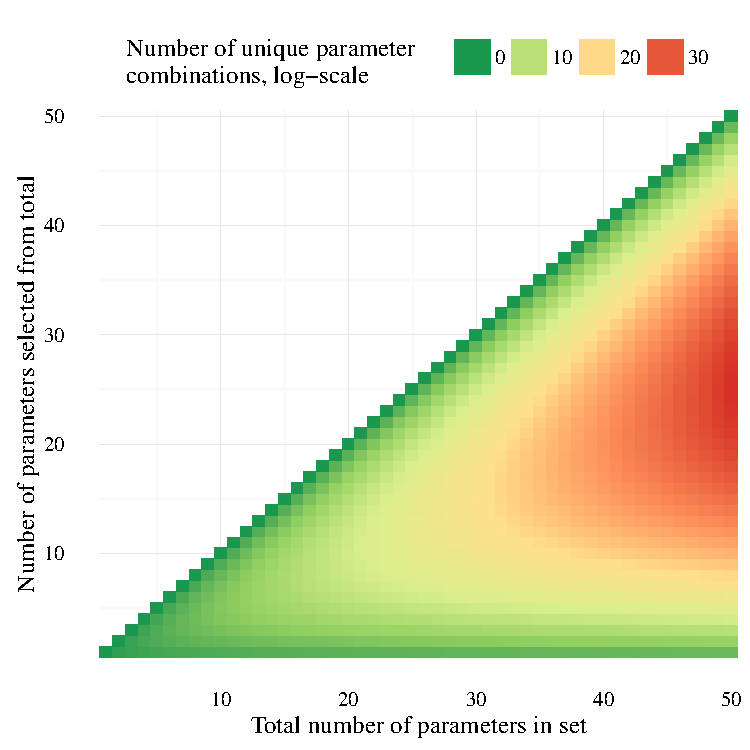
\includegraphics[width=0.6\textwidth]{figs/combnex-1} 

}

\caption[Examples of unique parameter combinations from different parameter sets and number of selected parameters]{Examples of unique parameter combinations from different parameter sets and number of selected parameters.  The number of combinations are shown for increasing numbers of selected parameters from the total in the set, where 50 parameter sets are shown each with one through 50 total parameters. Note that the number of unique combinations is shown as the natural-log.}\label{fig:combnex}
\end{figure}



% effects of changing initial and structural conditions
\begin{figure}[!ht]

{\centering 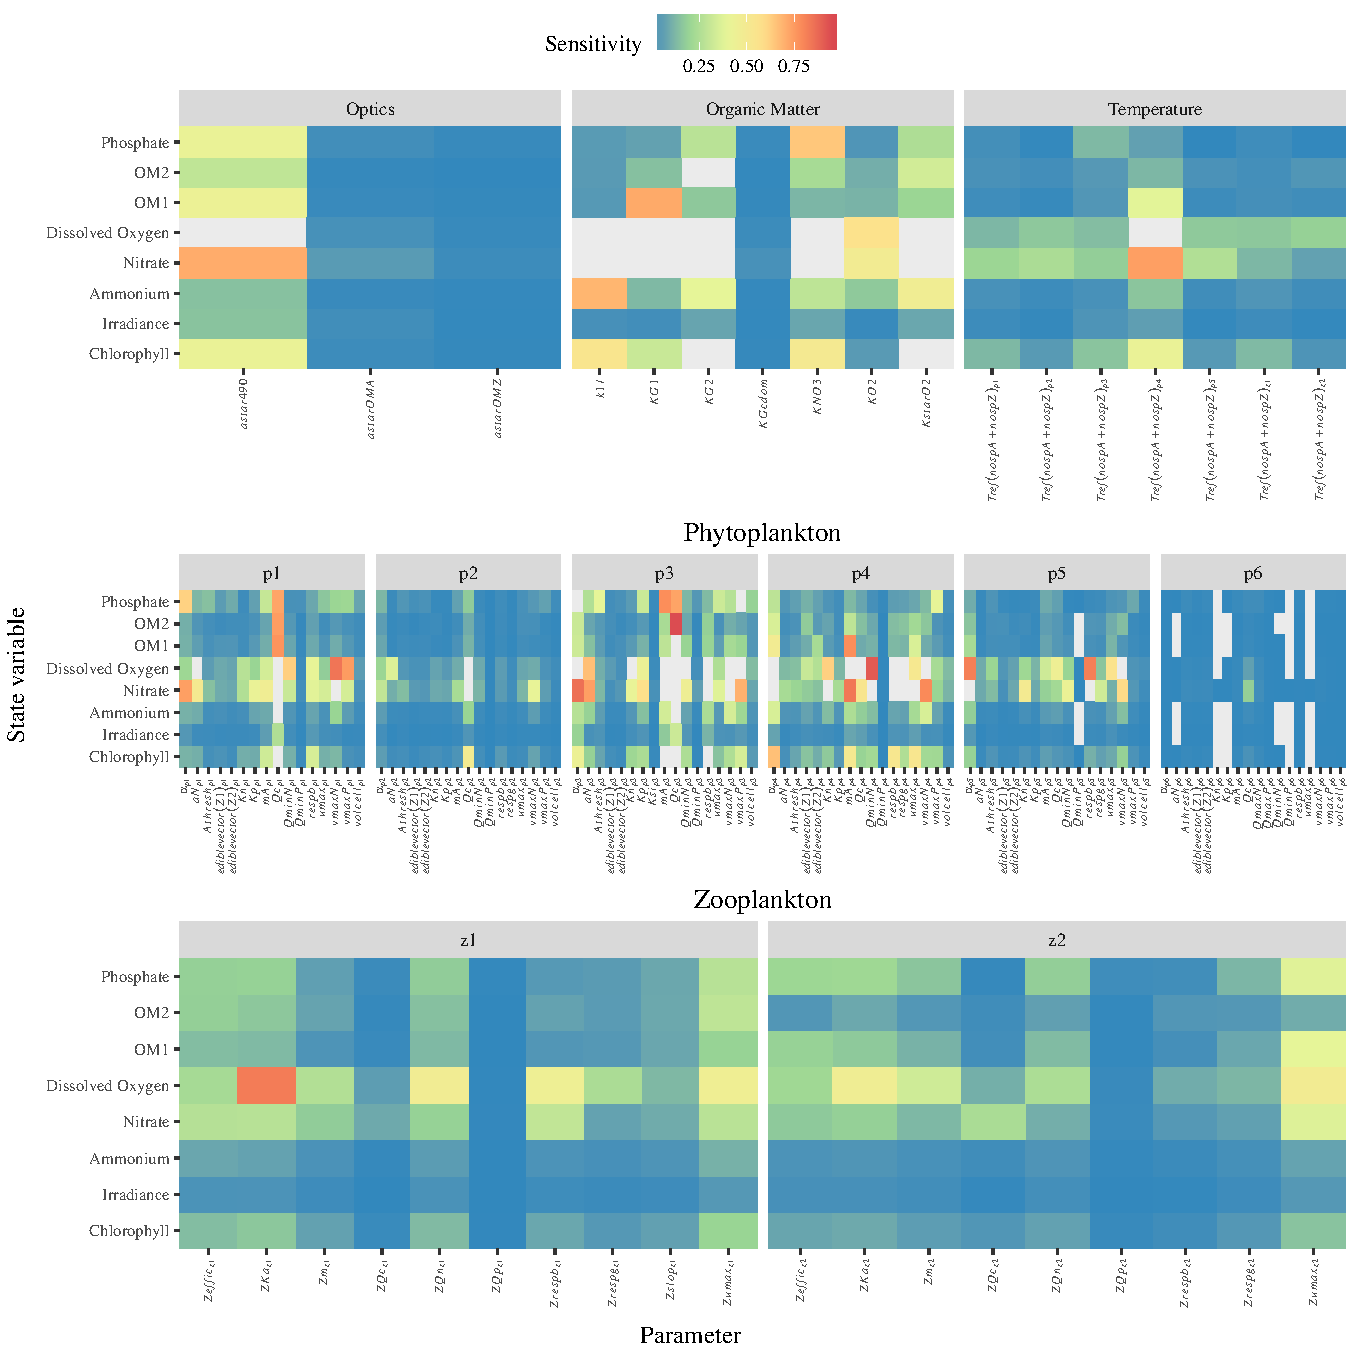
\includegraphics[width=\textwidth]{figs/sensalltile-1} 

}

\caption{Sensitivity values (L1, \cref{l1}) of all state variables to changes in parameter values using default conditions, changes in initial conditions (April, September seasonal means, \cref{tab:inits}), and changes in structural complexity (\cref{tab:strcs}). Parameters are grouped by category: optics, organic matter, phytoplankton, zooplankton, temperature, and zoplankton.  See \cref{tab:dosens} for L1 values for \ac{do} and \cref{tab:nh4sens,tab:chlsens,tab:irrsens,tab:no3sens,tab:om1sens,tab:om2sens,tab:po4sens} for the other state variables.}\label{fig:sensalltile}
\end{figure}



% identifiability plot
\begin{figure}[!ht]

{\centering 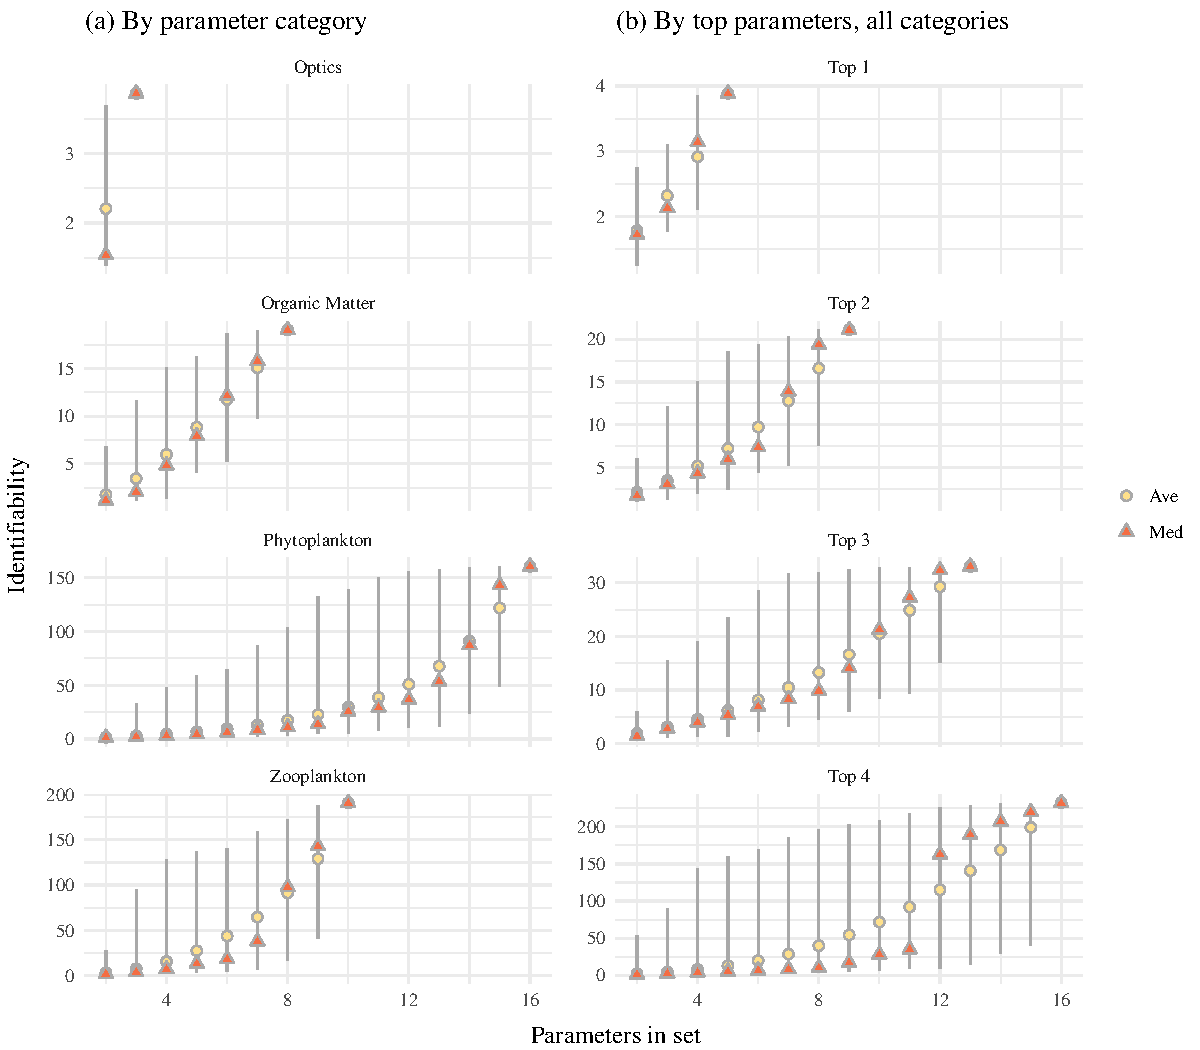
\includegraphics[width=\maxwidth]{figs/identplo-1} 

}

\caption{Identifiability (as $\gamma$, \cref{gameq}) of parameter subsets for \ac{do}.  Plots in (a) show identifiability by parameter categories and (b) shows identifiability by selecting the top 1 through 4 parameters in all categories.  Lines represent identifiability ranges for the possible combinations given the number of parameters in the set.  The temperature category is not shown because \ac{do} was sensitive to only one parameter (i.e., $\gamma = 1$).}\label{fig:identplo}
\end{figure}



% identifiability plot, all state variables
\begin{figure}[!ht]

{\centering 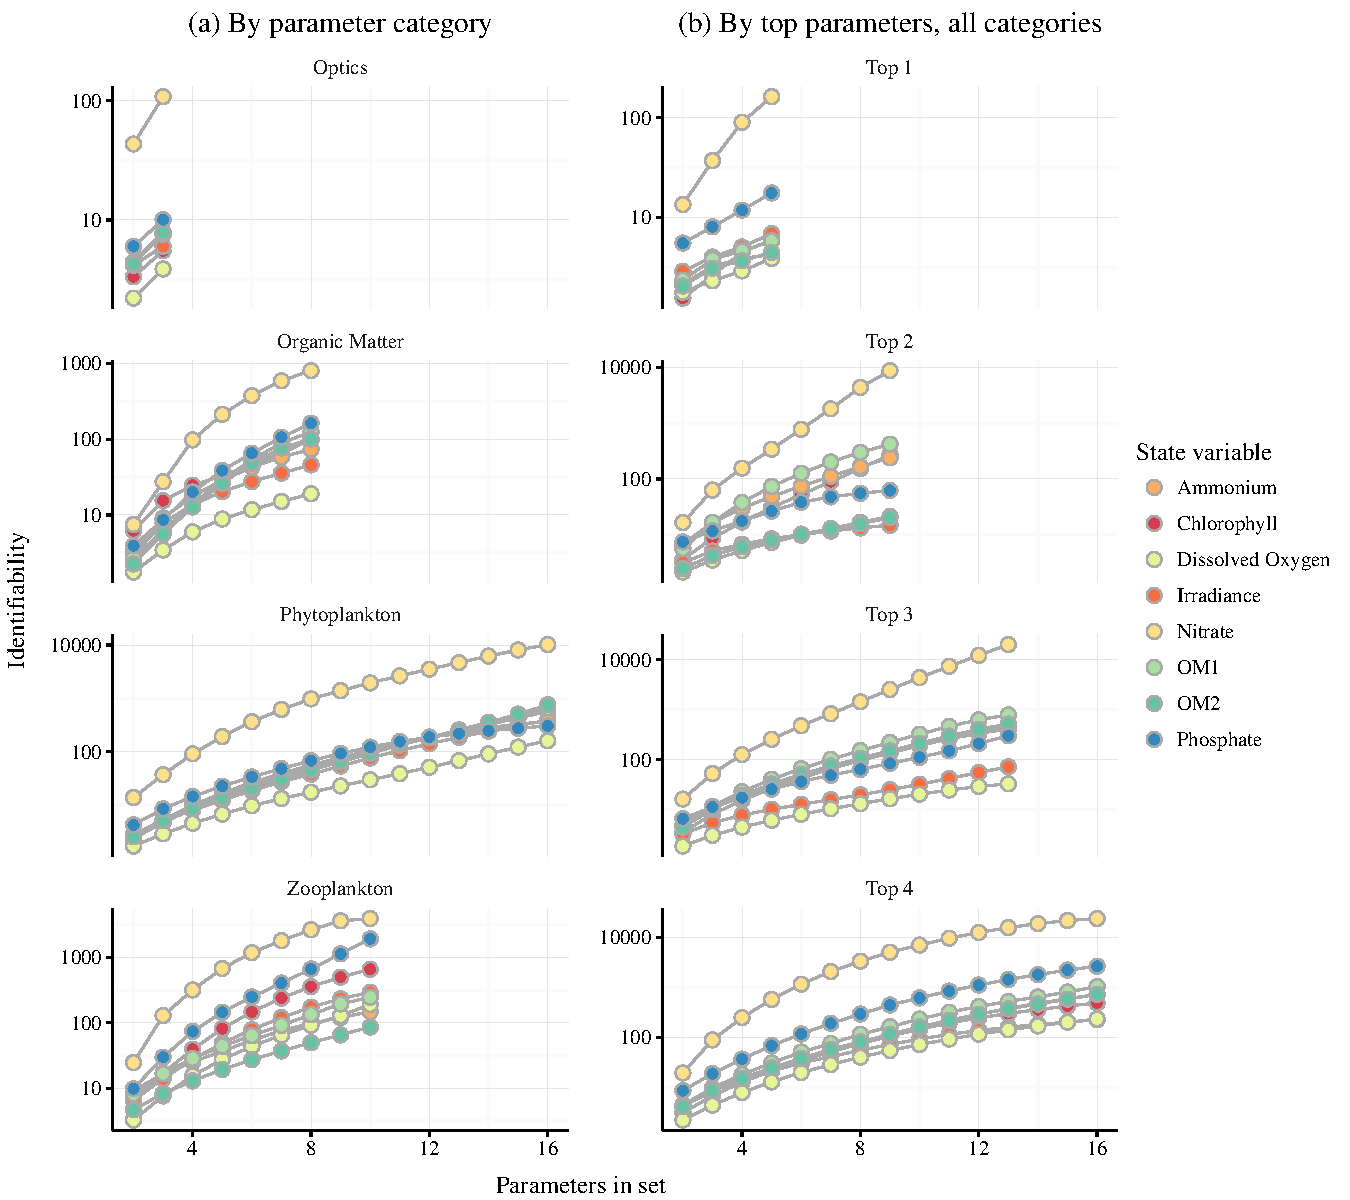
\includegraphics[width=\maxwidth]{figs/identploall-1} 

}

\caption[Average identifiability (as $\gamma$, \cref{gameq}) of parameter subsets for all state variables]{Average identifiability (as $\gamma$, \cref{gameq}) of parameter subsets for all state variables.  Plots in (a) show identifiability by parameter categories and (b) shows identifiability by selecting the top 1 through 4 parameters in all categories.  Identifiability was averaged for all combinations in a parameter set to evaluate relative differenes between state variables.  The temperature category is not shown because all state variables were sensitive to only one parameter (i.e., $\gamma = 1$).}\label{fig:identploall}
\end{figure}



% percent below gamma thresholds
\begin{figure}[!ht]

{\centering 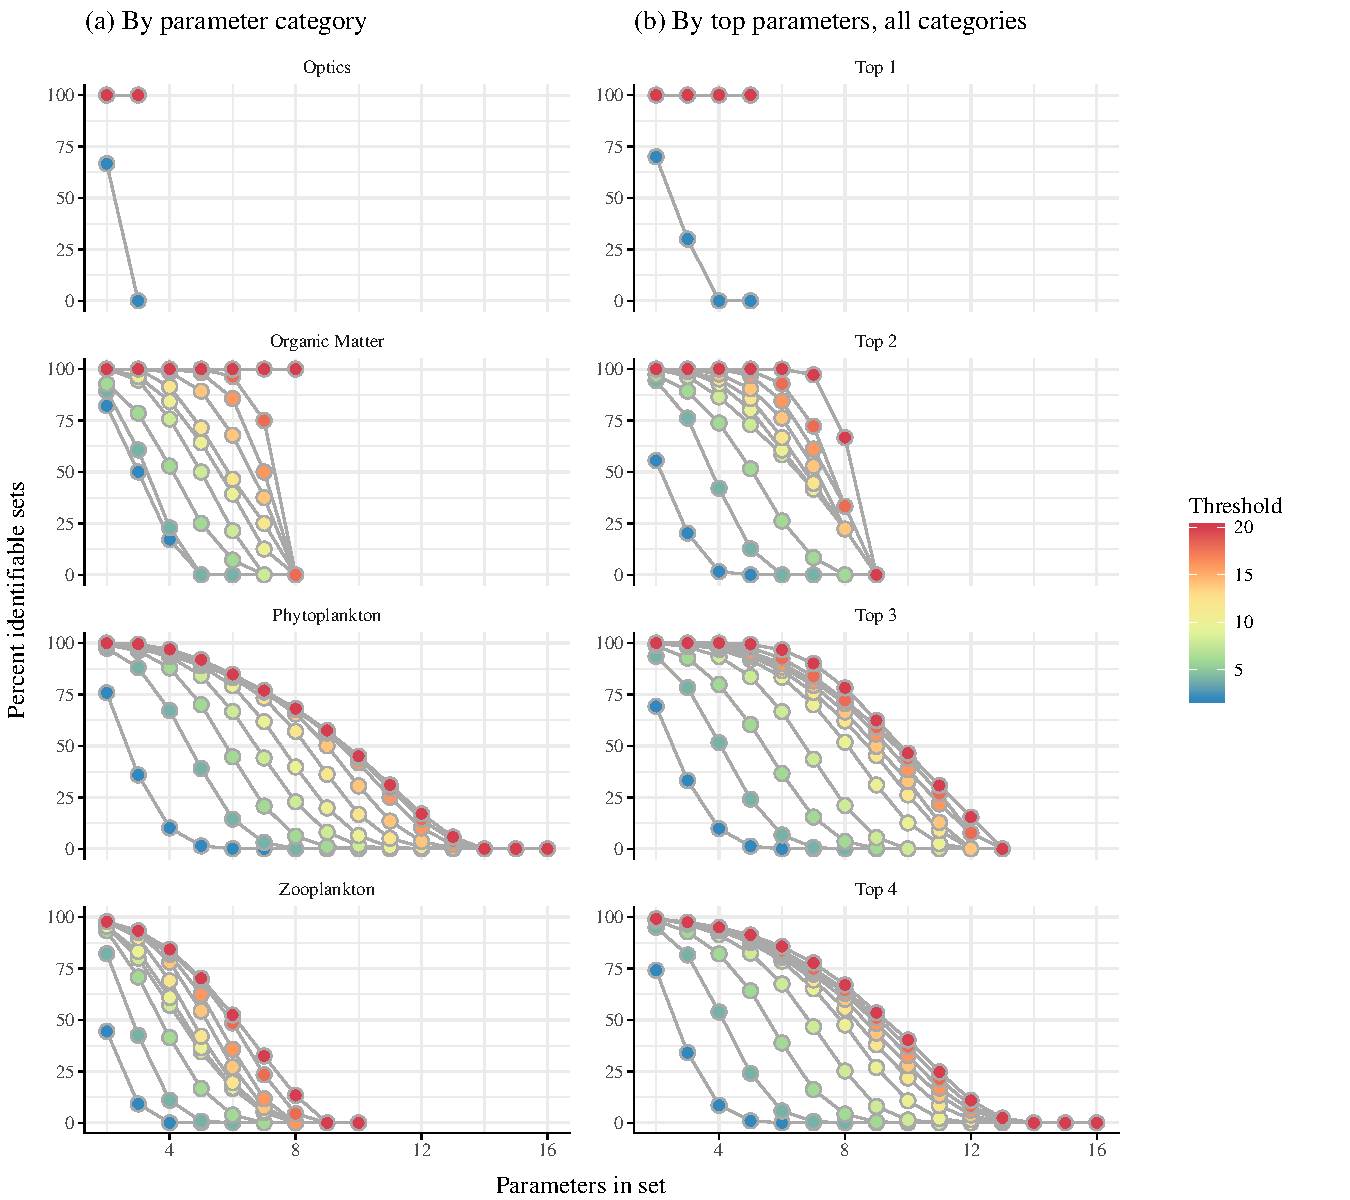
\includegraphics[width=\maxwidth]{figs/percthresh-1} 

}

\caption{Percent of identifiable parameter sets for \ac{do} at different $\gamma$ thresholds, selection criteria, and total number of parameters in the set.  Thresholds varied from $\gamma = 2$ to $20$ such that sets with $\gamma$ below a threshold were considered identifiable relative to the value. Plots in (a) show percent of identifiable sets by selecting parameters within categories and (b) shows percent identifiable by selecting from the top 1 through 4 parameters in all categories.  Percent identifiable was based on all sets in \cref{fig:identplo}.}\label{fig:percthresh}
\end{figure}



% parameter exclusion temp
\begin{figure}[!ht]

{\centering 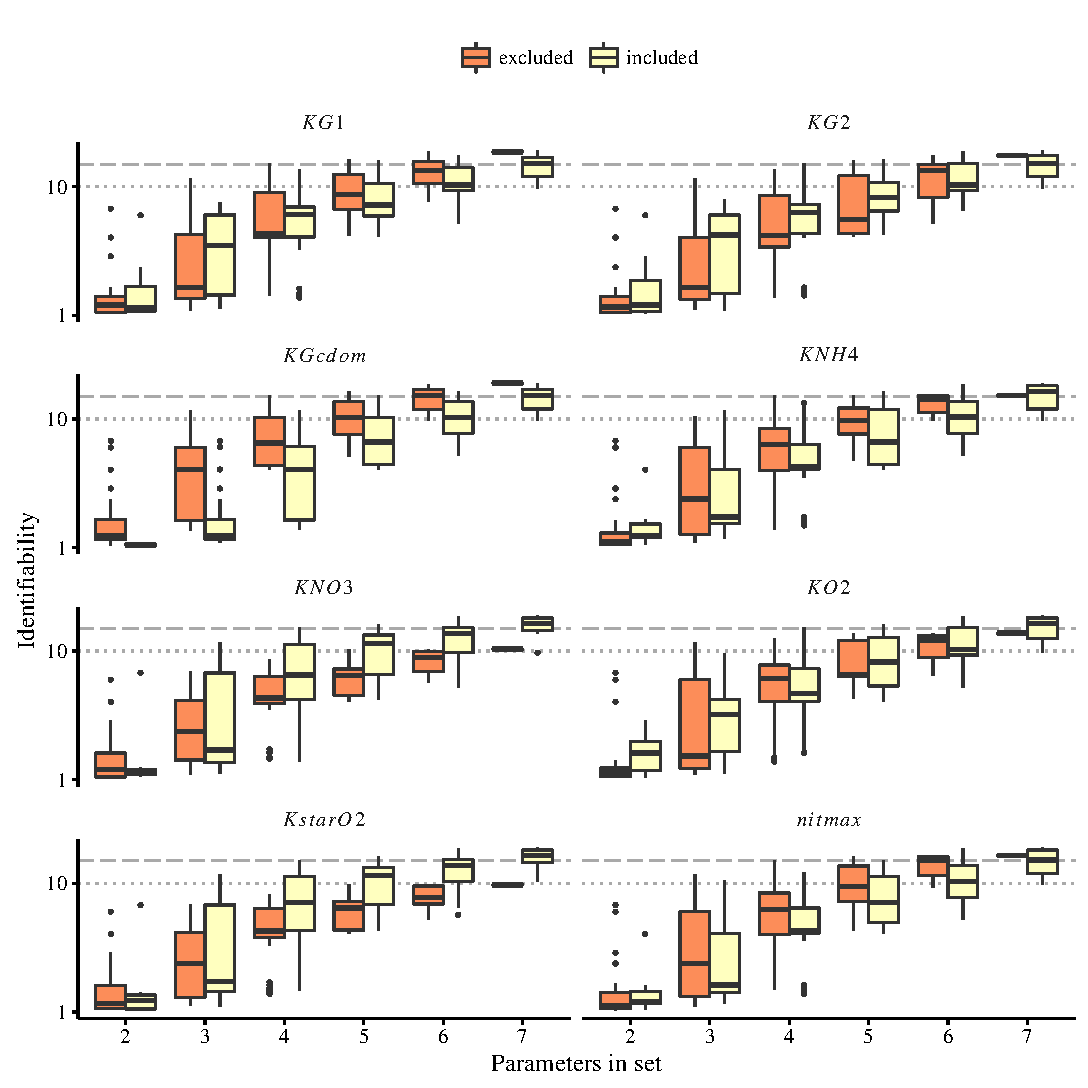
\includegraphics[width=\textwidth]{figs/exclex-1} 

}

\caption{Identifiability (as $\gamma$, \cref{gameq}) for \ac{do} of organic matter parameters for subset combinations in \cref{fig:identplo}.  Identifiability is evaluated for subsets that excluded and included the parameters at the top of each plot. Identifiability of including all eight parameters is in \cref{fig:identplo}. Grey lines indicate potential thresholds at $\gamma = 10, 15$ for maximum acceptable identifiability.}\label{fig:exclex}
\end{figure}



% heuristic plots, all state
\begin{figure}[!ht]

{\centering 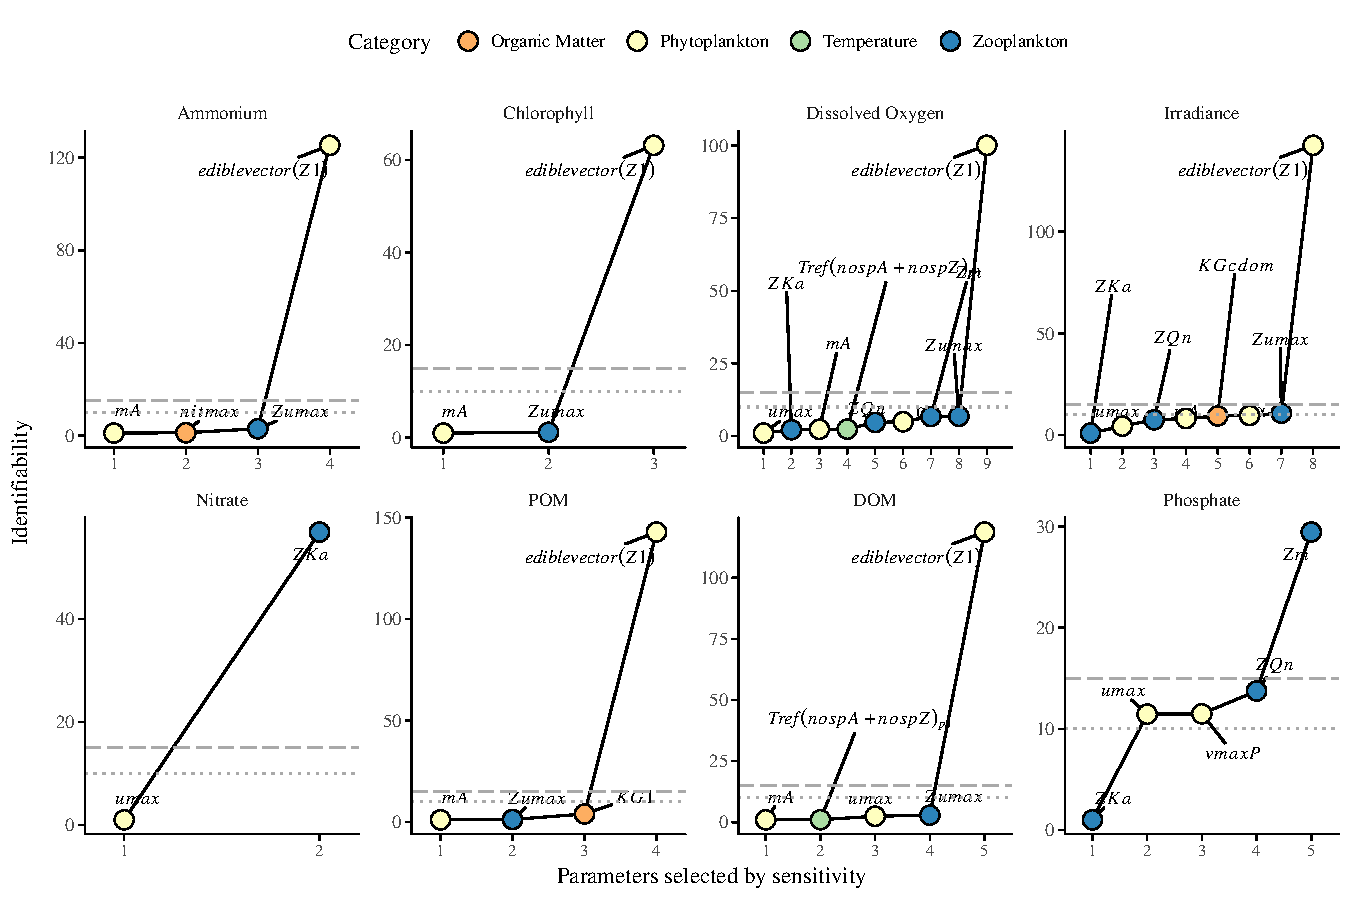
\includegraphics[width=\textwidth]{figs/heurist_stts-1} 

}

\caption[Identifiability (as ]{Identifiability (as $\gamma$, \cref{gameq}) of selecting parameters for all state variables. Parameters are selected by decreasing sensitivity independent of parameter categories. Grey lines indicate potential thresholds at $\gamma = 10, 15$ for maximum acceptable identifiability. Selection stops after $\gamma > 15$.}\label{fig:heurist_stts}
\end{figure}



% summary of initial/structural changes on parameter sensitivity
\begin{figure}[!ht]

{\centering 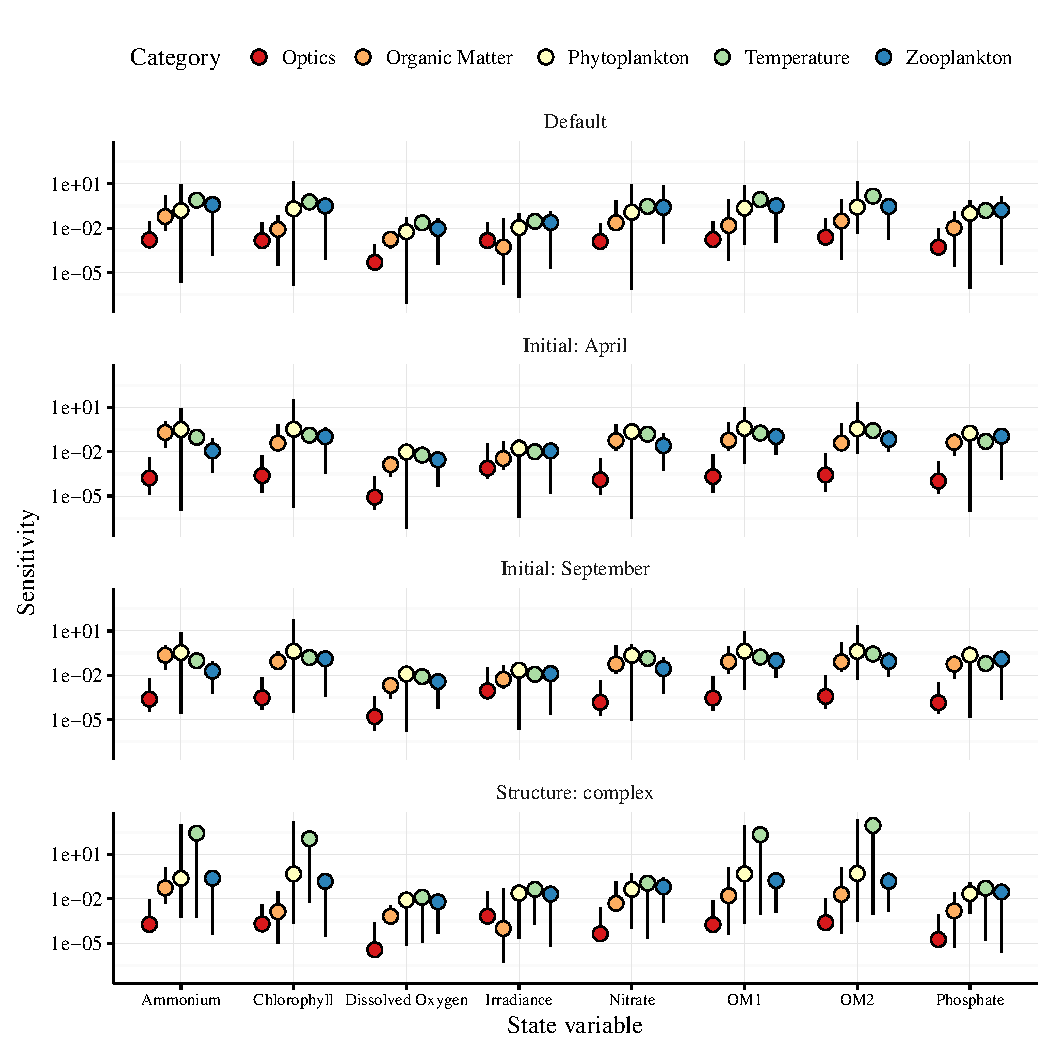
\includegraphics[width=\textwidth]{figs/inistrsumm-1} 

}

\caption{Summaries of changes in parameter sensitivity values (L1, \cref{l1}) from the default model conditions.  Sensitivity was re-evaluated using initial conditions as seasonal means for April and September, and added structural complexity.  Sensitivity is summarized as the minimum, median, and maximum for each state variable separated by parameter categories. Changes in average sensitivity from the default model conditions are in \cref{tab:inistrchg}.}\label{fig:inistrsumm}
\end{figure}



\clearpage

% supplementary material
\beginsupplement

%%
% sup tabs

% ammonium sensitivity all categories
%latex.default(totab, file = "", rowlabel = "Description", caption = cap.val,     caption.loc = "top", rowname = Description, rgroup = unique(cats),     n.rgroup = as.numeric(table(cats)), size = tabsize, label = paste0("tab:",         tablab), insert.bottom = foot.val)%
\begin{table}[!tbp]
{\footnotesize
\caption{Sensitivity of ammonium to perturbations of individual parameters.  Sensitivities are based on a 50\% increase from the initial parameter value, where $L1$ summarizes differences in model output from the default (see \cref{l1}).  Parameters that did not affect ammonium are not shown.  Parameters are grouped by categories as optics, temperature, phytoplankton, zooplankton, and organic matter.\label{tab:nh4sens}} 
\begin{center}
\begin{tabular}{lll}
\hline\hline
\multicolumn{1}{l}{Description}&\multicolumn{1}{c}{Parameter}&\multicolumn{1}{c}{L1}\tabularnewline
\hline
{\bfseries Optics}&&\tabularnewline
~~Chla specific absorption at 490 nm&\textit{astar490}&$0.03$\tabularnewline
~~OMA specific absorption at 490 nm&\textit{astarOMA}&$1.63\times 10^{-3}$\tabularnewline
~~OMZ specific absorption at 490 nm&\textit{astarOMZ}&$1.5\times 10^{-3}$\tabularnewline
\hline
{\bfseries Temperature}&&\tabularnewline
~~Optimum temperature for growth(C)&\textit{Tref(nospA+nospZ)$_{p1}$}&$0.79$\tabularnewline
\hline
{\bfseries Phytoplankton}&&\tabularnewline
~~mortality coefficient&\textit{mA}&$8.49$\tabularnewline
~~edibility vector for Z1&\textit{ediblevector(Z1)}&$1.32$\tabularnewline
~~maximum growth rate&\textit{umax}&$0.65$\tabularnewline
~~initial slope of the photosynthesis-irradiance relationship&\textit{alpha}&$0.6$\tabularnewline
~~N-uptake rate measured at umax&\textit{vmaxN}&$0.46$\tabularnewline
~~Phytoplankton threshold for grazing, is multiplied by VOLcell&\textit{Athresh}&$0.29$\tabularnewline
~~coefficient for non-limiting nutrient&\textit{aN}&$0.17$\tabularnewline
~~phytoplankton growth respiration coefficient&\textit{respg}&$0.16$\tabularnewline
~~phytoplankton basal respiration coefficient&\textit{respb}&$0.15$\tabularnewline
~~half-saturation constant for P&\textit{Kp}&$0.14$\tabularnewline
~~phytoplankton volume/cell&\textit{volcell}&$0.14$\tabularnewline
~~minimum N cell-quota&\textit{QminN}&$0.1$\tabularnewline
~~P-uptake rate measured at umax&\textit{vmaxP}&$0.1$\tabularnewline
~~phytoplankton carbon/cell&\textit{Qc}&$0.03$\tabularnewline
~~half-saturation constant for N&\textit{Kn}&$0.01$\tabularnewline
~~minimum P cell-quota&\textit{QminP}&$2.24\times 10^{-6}$\tabularnewline
\hline
{\bfseries Zooplankton}&&\tabularnewline
~~maximum growth rate of zooplankton&\textit{Zumax}&$1.42$\tabularnewline
~~assimilation efficiency as a fraction of ingestion&\textit{Zeffic}&$0.76$\tabularnewline
~~half saturation coefficient for grazing&\textit{ZKa}&$0.74$\tabularnewline
~~zooplankton nitrogen/individual&\textit{ZQn}&$0.62$\tabularnewline
~~Zooplankton mortality constant for quadratic mortality&\textit{Zm}&$0.5$\tabularnewline
~~proportion of grazed phytoplankton lost to sloppy feeding&\textit{Zslop}&$0.3$\tabularnewline
~~Zooplankton growth-dependent respiration factor&\textit{Zrespg}&$0.22$\tabularnewline
~~Zooplankton biomass-dependent respiration factor&\textit{Zrespb}&$0.16$\tabularnewline
~~zooplankton phosphorus/individual&\textit{ZQp}&$1.07\times 10^{-3}$\tabularnewline
~~zooplankton carbon/individual&\textit{ZQc}&$1.44\times 10^{-4}$\tabularnewline
\hline
{\bfseries Organic Matter}&&\tabularnewline
~~maximum rate of nitrification per day&\textit{nitmax}&$1.54$\tabularnewline
~~NH4 rate constant for nitrification&\textit{KNH4}&$0.66$\tabularnewline
~~turnover rate for OM1A and OM1Z&\textit{KG1}&$0.07$\tabularnewline
~~decay rate of CDOM, 1/day&\textit{KGcdom}&$0.07$\tabularnewline
~~half-saturation concentration for O2 utilization&\textit{KO2}&$0.06$\tabularnewline
~~O2 concentration that inhibits denitrification&\textit{KstarO2}&$0.05$\tabularnewline
~~turnover rate for OM2A and OM2Z&\textit{KG2}&$0.03$\tabularnewline
~~half-saturation concentration for NO3 used in denitrification&\textit{KNO3}&$7.55\times 10^{-3}$\tabularnewline
\hline
\end{tabular}\end{center}}

\end{table}


% chlorophyll sensitivity all categories
%latex.default(totab, file = "", rowlabel = "Description", caption = cap.val,     caption.loc = "top", rowname = Description, rgroup = unique(cats),     n.rgroup = as.numeric(table(cats)), size = tabsize, label = paste0("tab:",         tablab), insert.bottom = foot.val)%
\begin{table}[!tbp]
{\footnotesize
\caption{Sensitivity of \ac{chla} to perturbations of individual parameters.  Sensitivities are based on a 50\% increase from the initial parameter value, where $L1$ summarizes differences in model output from the default (see \cref{l1}).  Parameters that did not affect \ac{chla} are not shown.  Parameters are grouped by categories as optics, temperature, phytoplankton, zooplankton, and organic matter.\label{tab:chlsens}} 
\begin{center}
\begin{tabular}{lll}
\hline\hline
\multicolumn{1}{l}{Description}&\multicolumn{1}{c}{Parameter}&\multicolumn{1}{c}{L1}\tabularnewline
\hline
{\bfseries Optics}&&\tabularnewline
~~Chla specific absorption at 490 nm&\textit{astar490}&$0.02$\tabularnewline
~~OMA specific absorption at 490 nm&\textit{astarOMA}&$1.45\times 10^{-3}$\tabularnewline
~~OMZ specific absorption at 490 nm&\textit{astarOMZ}&$1.13\times 10^{-3}$\tabularnewline
\hline
{\bfseries Temperature}&&\tabularnewline
~~Optimum temperature for growth(C)&\textit{Tref(nospA+nospZ)$_{p1}$}&$0.6$\tabularnewline
\hline
{\bfseries Phytoplankton}&&\tabularnewline
~~mortality coefficient&\textit{mA}&$13.94$\tabularnewline
~~edibility vector for Z1&\textit{ediblevector(Z1)}&$0.95$\tabularnewline
~~maximum growth rate&\textit{umax}&$0.85$\tabularnewline
~~initial slope of the photosynthesis-irradiance relationship&\textit{alpha}&$0.62$\tabularnewline
~~N-uptake rate measured at umax&\textit{vmaxN}&$0.53$\tabularnewline
~~phytoplankton growth respiration coefficient&\textit{respg}&$0.26$\tabularnewline
~~Phytoplankton threshold for grazing, is multiplied by VOLcell&\textit{Athresh}&$0.25$\tabularnewline
~~phytoplankton basal respiration coefficient&\textit{respb}&$0.24$\tabularnewline
~~coefficient for non-limiting nutrient&\textit{aN}&$0.17$\tabularnewline
~~half-saturation constant for P&\textit{Kp}&$0.14$\tabularnewline
~~P-uptake rate measured at umax&\textit{vmaxP}&$0.12$\tabularnewline
~~phytoplankton volume/cell&\textit{volcell}&$0.1$\tabularnewline
~~minimum N cell-quota&\textit{QminN}&$0.07$\tabularnewline
~~phytoplankton carbon/cell&\textit{Qc}&$0.02$\tabularnewline
~~half-saturation constant for N&\textit{Kn}&$0.01$\tabularnewline
~~minimum P cell-quota&\textit{QminP}&$1.38\times 10^{-6}$\tabularnewline
\hline
{\bfseries Zooplankton}&&\tabularnewline
~~maximum growth rate of zooplankton&\textit{Zumax}&$1.02$\tabularnewline
~~half saturation coefficient for grazing&\textit{ZKa}&$0.85$\tabularnewline
~~assimilation efficiency as a fraction of ingestion&\textit{Zeffic}&$0.57$\tabularnewline
~~zooplankton nitrogen/individual&\textit{ZQn}&$0.52$\tabularnewline
~~Zooplankton mortality constant for quadratic mortality&\textit{Zm}&$0.41$\tabularnewline
~~proportion of grazed phytoplankton lost to sloppy feeding&\textit{Zslop}&$0.23$\tabularnewline
~~Zooplankton growth-dependent respiration factor&\textit{Zrespg}&$0.17$\tabularnewline
~~Zooplankton biomass-dependent respiration factor&\textit{Zrespb}&$0.14$\tabularnewline
~~zooplankton phosphorus/individual&\textit{ZQp}&$1.29\times 10^{-3}$\tabularnewline
~~zooplankton carbon/individual&\textit{ZQc}&$7.55\times 10^{-5}$\tabularnewline
\hline
{\bfseries Organic Matter}&&\tabularnewline
~~decay rate of CDOM, 1/day&\textit{KGcdom}&$0.07$\tabularnewline
~~turnover rate for OM1A and OM1Z&\textit{KG1}&$0.03$\tabularnewline
~~turnover rate for OM2A and OM2Z&\textit{KG2}&$0.01$\tabularnewline
~~O2 concentration that inhibits denitrification&\textit{KstarO2}&$0.01$\tabularnewline
~~half-saturation concentration for O2 utilization&\textit{KO2}&$3.35\times 10^{-3}$\tabularnewline
~~half-saturation concentration for NO3 used in denitrification&\textit{KNO3}&$1.19\times 10^{-3}$\tabularnewline
~~maximum rate of nitrification per day&\textit{nitmax}&$3.4\times 10^{-5}$\tabularnewline
~~NH4 rate constant for nitrification&\textit{KNH4}&$2.97\times 10^{-5}$\tabularnewline
\hline
\end{tabular}\end{center}}

\end{table}


% irradiance sensitivity all categories
%latex.default(totab, file = "", rowlabel = "Description", caption = cap.val,     caption.loc = "top", rowname = Description, rgroup = unique(cats),     n.rgroup = as.numeric(table(cats)), size = tabsize, label = paste0("tab:",         tablab), insert.bottom = foot.val)%
\begin{table}[!tbp]
{\footnotesize
\caption{Sensitivity of irradiance to perturbations of individual parameters.  Sensitivities are based on a 50\% increase from the initial parameter value, where $L1$ summarizes differences in model output from the default (see \cref{l1}).  Parameters that did not affect irradiance are not shown.  Parameters are grouped by categories as optics, temperature, phytoplankton, zooplankton, and organic matter.\label{tab:irrsens}} 
\begin{center}
\begin{tabular}{lll}
\hline\hline
\multicolumn{1}{l}{Description}&\multicolumn{1}{c}{Parameter}&\multicolumn{1}{c}{L1}\tabularnewline
\hline
{\bfseries Optics}&&\tabularnewline
~~Chla specific absorption at 490 nm&\textit{astar490}&$0.02$\tabularnewline
~~OMA specific absorption at 490 nm&\textit{astarOMA}&$1.47\times 10^{-3}$\tabularnewline
~~OMZ specific absorption at 490 nm&\textit{astarOMZ}&$1.34\times 10^{-3}$\tabularnewline
\hline
{\bfseries Temperature}&&\tabularnewline
~~Optimum temperature for growth(C)&\textit{Tref(nospA+nospZ)$_{p1}$}&$0.03$\tabularnewline
\hline
{\bfseries Phytoplankton}&&\tabularnewline
~~maximum growth rate&\textit{umax}&$0.09$\tabularnewline
~~mortality coefficient&\textit{mA}&$0.05$\tabularnewline
~~initial slope of the photosynthesis-irradiance relationship&\textit{alpha}&$0.04$\tabularnewline
~~edibility vector for Z1&\textit{ediblevector(Z1)}&$0.04$\tabularnewline
~~N-uptake rate measured at umax&\textit{vmaxN}&$0.03$\tabularnewline
~~Phytoplankton threshold for grazing, is multiplied by VOLcell&\textit{Athresh}&$0.02$\tabularnewline
~~coefficient for non-limiting nutrient&\textit{aN}&$0.01$\tabularnewline
~~phytoplankton growth respiration coefficient&\textit{respg}&$0.01$\tabularnewline
~~half-saturation constant for P&\textit{Kp}&$0.01$\tabularnewline
~~P-uptake rate measured at umax&\textit{vmaxP}&$9.48\times 10^{-3}$\tabularnewline
~~phytoplankton basal respiration coefficient&\textit{respb}&$9.38\times 10^{-3}$\tabularnewline
~~phytoplankton volume/cell&\textit{volcell}&$8.1\times 10^{-3}$\tabularnewline
~~minimum N cell-quota&\textit{QminN}&$5.75\times 10^{-3}$\tabularnewline
~~phytoplankton carbon/cell&\textit{Qc}&$3.78\times 10^{-3}$\tabularnewline
~~half-saturation constant for N&\textit{Kn}&$9.81\times 10^{-4}$\tabularnewline
~~minimum P cell-quota&\textit{QminP}&$1.92\times 10^{-7}$\tabularnewline
\hline
{\bfseries Zooplankton}&&\tabularnewline
~~half saturation coefficient for grazing&\textit{ZKa}&$0.13$\tabularnewline
~~zooplankton nitrogen/individual&\textit{ZQn}&$0.06$\tabularnewline
~~maximum growth rate of zooplankton&\textit{Zumax}&$0.04$\tabularnewline
~~Zooplankton mortality constant for quadratic mortality&\textit{Zm}&$0.04$\tabularnewline
~~assimilation efficiency as a fraction of ingestion&\textit{Zeffic}&$0.03$\tabularnewline
~~proportion of grazed phytoplankton lost to sloppy feeding&\textit{Zslop}&$0.02$\tabularnewline
~~Zooplankton growth-dependent respiration factor&\textit{Zrespg}&$0.01$\tabularnewline
~~Zooplankton biomass-dependent respiration factor&\textit{Zrespb}&$9.67\times 10^{-3}$\tabularnewline
~~zooplankton phosphorus/individual&\textit{ZQp}&$9.34\times 10^{-5}$\tabularnewline
~~zooplankton carbon/individual&\textit{ZQc}&$1.99\times 10^{-5}$\tabularnewline
\hline
{\bfseries Organic Matter}&&\tabularnewline
~~decay rate of CDOM, 1/day&\textit{KGcdom}&$0.05$\tabularnewline
~~turnover rate for OM1A and OM1Z&\textit{KG1}&$3.96\times 10^{-3}$\tabularnewline
~~turnover rate for OM2A and OM2Z&\textit{KG2}&$9.88\times 10^{-4}$\tabularnewline
~~O2 concentration that inhibits denitrification&\textit{KstarO2}&$7.2\times 10^{-4}$\tabularnewline
~~half-saturation concentration for O2 utilization&\textit{KO2}&$3.54\times 10^{-4}$\tabularnewline
~~half-saturation concentration for NO3 used in denitrification&\textit{KNO3}&$6.18\times 10^{-5}$\tabularnewline
~~maximum rate of nitrification per day&\textit{nitmax}&$1.72\times 10^{-6}$\tabularnewline
~~NH4 rate constant for nitrification&\textit{KNH4}&$1.48\times 10^{-6}$\tabularnewline
\hline
\end{tabular}\end{center}}

\end{table}


% nitrate sensitivity all categories
%latex.default(totab, file = "", rowlabel = "Description", caption = cap.val,     caption.loc = "top", rowname = Description, rgroup = unique(cats),     n.rgroup = as.numeric(table(cats)), size = tabsize, label = paste0("tab:",         tablab), insert.bottom = foot.val)%
\begin{table}[!tbp]
{\footnotesize
\caption{Sensitivity of nitrate to perturbations of individual parameters.  Sensitivities are based on a 50\% increase from the initial parameter value, where $L1$ summarizes differences in model output from the default (see \cref{l1}).  Parameters that did not affect nitrate are not shown.  Parameters are grouped by categories as optics, temperature, phytoplankton, zooplankton, and organic matter.\label{tab:no3sens}} 
\begin{center}
\begin{tabular}{lll}
\hline\hline
\multicolumn{1}{l}{Description}&\multicolumn{1}{c}{Parameter}&\multicolumn{1}{c}{L1}\tabularnewline
\hline
{\bfseries Optics}&&\tabularnewline
~~Chla specific absorption at 490 nm&\textit{astar490}&$0.02$\tabularnewline
~~OMZ specific absorption at 490 nm&\textit{astarOMZ}&$1.27\times 10^{-3}$\tabularnewline
~~OMA specific absorption at 490 nm&\textit{astarOMA}&$1.19\times 10^{-3}$\tabularnewline
\hline
{\bfseries Temperature}&&\tabularnewline
~~Optimum temperature for growth(C)&\textit{Tref(nospA+nospZ)$_{p1}$}&$0.3$\tabularnewline
\hline
{\bfseries Phytoplankton}&&\tabularnewline
~~maximum growth rate&\textit{umax}&$8.49$\tabularnewline
~~phytoplankton carbon/cell&\textit{Qc}&$0.89$\tabularnewline
~~initial slope of the photosynthesis-irradiance relationship&\textit{alpha}&$0.7$\tabularnewline
~~edibility vector for Z1&\textit{ediblevector(Z1)}&$0.33$\tabularnewline
~~mortality coefficient&\textit{mA}&$0.27$\tabularnewline
~~Phytoplankton threshold for grazing, is multiplied by VOLcell&\textit{Athresh}&$0.2$\tabularnewline
~~N-uptake rate measured at umax&\textit{vmaxN}&$0.19$\tabularnewline
~~coefficient for non-limiting nutrient&\textit{aN}&$0.13$\tabularnewline
~~phytoplankton growth respiration coefficient&\textit{respg}&$0.11$\tabularnewline
~~phytoplankton volume/cell&\textit{volcell}&$0.1$\tabularnewline
~~P-uptake rate measured at umax&\textit{vmaxP}&$0.1$\tabularnewline
~~half-saturation constant for P&\textit{Kp}&$0.09$\tabularnewline
~~minimum N cell-quota&\textit{QminN}&$0.09$\tabularnewline
~~phytoplankton basal respiration coefficient&\textit{respb}&$0.07$\tabularnewline
~~half-saturation constant for N&\textit{Kn}&$7.06\times 10^{-3}$\tabularnewline
~~minimum P cell-quota&\textit{QminP}&$6.67\times 10^{-7}$\tabularnewline
\hline
{\bfseries Zooplankton}&&\tabularnewline
~~half saturation coefficient for grazing&\textit{ZKa}&$7.59$\tabularnewline
~~zooplankton nitrogen/individual&\textit{ZQn}&$1.17$\tabularnewline
~~Zooplankton mortality constant for quadratic mortality&\textit{Zm}&$0.7$\tabularnewline
~~maximum growth rate of zooplankton&\textit{Zumax}&$0.34$\tabularnewline
~~proportion of grazed phytoplankton lost to sloppy feeding&\textit{Zslop}&$0.26$\tabularnewline
~~assimilation efficiency as a fraction of ingestion&\textit{Zeffic}&$0.25$\tabularnewline
~~Zooplankton growth-dependent respiration factor&\textit{Zrespg}&$0.17$\tabularnewline
~~Zooplankton biomass-dependent respiration factor&\textit{Zrespb}&$0.1$\tabularnewline
~~zooplankton carbon/individual&\textit{ZQc}&$3.8\times 10^{-3}$\tabularnewline
~~zooplankton phosphorus/individual&\textit{ZQp}&$8.59\times 10^{-4}$\tabularnewline
\hline
{\bfseries Organic Matter}&&\tabularnewline
~~O2 concentration that inhibits denitrification&\textit{KstarO2}&$0.78$\tabularnewline
~~half-saturation concentration for NO3 used in denitrification&\textit{KNO3}&$0.07$\tabularnewline
~~decay rate of CDOM, 1/day&\textit{KGcdom}&$0.04$\tabularnewline
~~half-saturation concentration for O2 utilization&\textit{KO2}&$0.03$\tabularnewline
~~turnover rate for OM1A and OM1Z&\textit{KG1}&$0.02$\tabularnewline
~~turnover rate for OM2A and OM2Z&\textit{KG2}&$0.01$\tabularnewline
~~maximum rate of nitrification per day&\textit{nitmax}&$9.96\times 10^{-3}$\tabularnewline
~~NH4 rate constant for nitrification&\textit{KNH4}&$9.87\times 10^{-3}$\tabularnewline
\hline
\end{tabular}\end{center}}

\end{table}


% om1 sensitivity all categories
%latex.default(totab, file = "", rowlabel = "Description", caption = cap.val,     caption.loc = "top", rowname = Description, rgroup = unique(cats),     n.rgroup = as.numeric(table(cats)), size = tabsize, label = paste0("tab:",         tablab), insert.bottom = foot.val)%
\begin{table}[!tbp]
{\footnotesize
\caption{Sensitivity of \ac{pom} to perturbations of individual parameters.  Sensitivities are based on a 50\% increase from the initial parameter value, where $L1$ summarizes differences in model output from the default (see \cref{l1}).  Parameters that did not affect \ac{pom} are not shown.  Parameters are grouped by categories as optics, temperature, phytoplankton, zooplankton, and organic matter.\label{tab:om1sens}} 
\begin{center}
\begin{tabular}{lll}
\hline\hline
\multicolumn{1}{l}{Description}&\multicolumn{1}{c}{Parameter}&\multicolumn{1}{c}{L1}\tabularnewline
\hline
{\bfseries Optics}&&\tabularnewline
~~Chla specific absorption at 490 nm&\textit{astar490}&$0.03$\tabularnewline
~~OMA specific absorption at 490 nm&\textit{astarOMA}&$1.73\times 10^{-3}$\tabularnewline
~~OMZ specific absorption at 490 nm&\textit{astarOMZ}&$1.49\times 10^{-3}$\tabularnewline
\hline
{\bfseries Temperature}&&\tabularnewline
~~Optimum temperature for growth(C)&\textit{Tref(nospA+nospZ)$_{p1}$}&$0.86$\tabularnewline
\hline
{\bfseries Phytoplankton}&&\tabularnewline
~~mortality coefficient&\textit{mA}&$7.22$\tabularnewline
~~edibility vector for Z1&\textit{ediblevector(Z1)}&$0.9$\tabularnewline
~~maximum growth rate&\textit{umax}&$0.89$\tabularnewline
~~phytoplankton carbon/cell&\textit{Qc}&$0.67$\tabularnewline
~~initial slope of the photosynthesis-irradiance relationship&\textit{alpha}&$0.67$\tabularnewline
~~N-uptake rate measured at umax&\textit{vmaxN}&$0.45$\tabularnewline
~~phytoplankton growth respiration coefficient&\textit{respg}&$0.29$\tabularnewline
~~phytoplankton basal respiration coefficient&\textit{respb}&$0.24$\tabularnewline
~~Phytoplankton threshold for grazing, is multiplied by VOLcell&\textit{Athresh}&$0.22$\tabularnewline
~~minimum N cell-quota&\textit{QminN}&$0.21$\tabularnewline
~~coefficient for non-limiting nutrient&\textit{aN}&$0.14$\tabularnewline
~~half-saturation constant for P&\textit{Kp}&$0.11$\tabularnewline
~~phytoplankton volume/cell&\textit{volcell}&$0.1$\tabularnewline
~~P-uptake rate measured at umax&\textit{vmaxP}&$0.09$\tabularnewline
~~half-saturation constant for N&\textit{Kn}&$0.01$\tabularnewline
~~minimum P cell-quota&\textit{QminP}&$7.35\times 10^{-4}$\tabularnewline
\hline
{\bfseries Zooplankton}&&\tabularnewline
~~maximum growth rate of zooplankton&\textit{Zumax}&$0.96$\tabularnewline
~~half saturation coefficient for grazing&\textit{ZKa}&$0.79$\tabularnewline
~~assimilation efficiency as a fraction of ingestion&\textit{Zeffic}&$0.54$\tabularnewline
~~zooplankton nitrogen/individual&\textit{ZQn}&$0.49$\tabularnewline
~~Zooplankton mortality constant for quadratic mortality&\textit{Zm}&$0.39$\tabularnewline
~~proportion of grazed phytoplankton lost to sloppy feeding&\textit{Zslop}&$0.27$\tabularnewline
~~Zooplankton growth-dependent respiration factor&\textit{Zrespg}&$0.16$\tabularnewline
~~Zooplankton biomass-dependent respiration factor&\textit{Zrespb}&$0.12$\tabularnewline
~~zooplankton carbon/individual&\textit{ZQc}&$9.64\times 10^{-3}$\tabularnewline
~~zooplankton phosphorus/individual&\textit{ZQp}&$1.06\times 10^{-3}$\tabularnewline
\hline
{\bfseries Organic Matter}&&\tabularnewline
~~turnover rate for OM1A and OM1Z&\textit{KG1}&$0.92$\tabularnewline
~~decay rate of CDOM, 1/day&\textit{KGcdom}&$0.07$\tabularnewline
~~half-saturation concentration for O2 utilization&\textit{KO2}&$0.04$\tabularnewline
~~O2 concentration that inhibits denitrification&\textit{KstarO2}&$0.02$\tabularnewline
~~turnover rate for OM2A and OM2Z&\textit{KG2}&$0.01$\tabularnewline
~~half-saturation concentration for NO3 used in denitrification&\textit{KNO3}&$3.72\times 10^{-3}$\tabularnewline
~~maximum rate of nitrification per day&\textit{nitmax}&$6.98\times 10^{-5}$\tabularnewline
~~NH4 rate constant for nitrification&\textit{KNH4}&$6.41\times 10^{-5}$\tabularnewline
\hline
\end{tabular}\end{center}}

\end{table}


% om2 sensitivity all categories
%latex.default(totab, file = "", rowlabel = "Description", caption = cap.val,     caption.loc = "top", rowname = Description, rgroup = unique(cats),     n.rgroup = as.numeric(table(cats)), size = tabsize, label = paste0("tab:",         tablab), insert.bottom = foot.val)%
\begin{table}[!tbp]
{\footnotesize
\caption{Sensitivity of \acl{dom} to perturbations of individual parameters.  Sensitivities are based on a 50\% increase from the initial parameter value, where $L1$ summarizes differences in model output from the default (see \cref{l1}).  Parameters that did not affect \acl{dom} are not shown.  Parameters are grouped by categories as optics, temperature, phytoplankton, zooplankton, and organic matter.\label{tab:om2sens}} 
\begin{center}
\begin{tabular}{lll}
\hline\hline
\multicolumn{1}{l}{Description}&\multicolumn{1}{c}{Parameter}&\multicolumn{1}{c}{L1}\tabularnewline
\hline
{\bfseries Optics}&&\tabularnewline
~~Chla specific absorption at 490 nm&\textit{astar490}&$0.04$\tabularnewline
~~OMA specific absorption at 490 nm&\textit{astarOMA}&$2.48\times 10^{-3}$\tabularnewline
~~OMZ specific absorption at 490 nm&\textit{astarOMZ}&$2.04\times 10^{-3}$\tabularnewline
\hline
{\bfseries Temperature}&&\tabularnewline
~~Optimum temperature for growth(C)&\textit{Tref(nospA+nospZ)$_{p1}$}&$1.48$\tabularnewline
\hline
{\bfseries Phytoplankton}&&\tabularnewline
~~mortality coefficient&\textit{mA}&$14.25$\tabularnewline
~~maximum growth rate&\textit{umax}&$1.11$\tabularnewline
~~edibility vector for Z1&\textit{ediblevector(Z1)}&$0.94$\tabularnewline
~~N-uptake rate measured at umax&\textit{vmaxN}&$0.86$\tabularnewline
~~initial slope of the photosynthesis-irradiance relationship&\textit{alpha}&$0.85$\tabularnewline
~~phytoplankton carbon/cell&\textit{Qc}&$0.67$\tabularnewline
~~phytoplankton growth respiration coefficient&\textit{respg}&$0.36$\tabularnewline
~~phytoplankton basal respiration coefficient&\textit{respb}&$0.29$\tabularnewline
~~coefficient for non-limiting nutrient&\textit{aN}&$0.25$\tabularnewline
~~minimum N cell-quota&\textit{QminN}&$0.24$\tabularnewline
~~Phytoplankton threshold for grazing, is multiplied by VOLcell&\textit{Athresh}&$0.22$\tabularnewline
~~half-saturation constant for P&\textit{Kp}&$0.2$\tabularnewline
~~P-uptake rate measured at umax&\textit{vmaxP}&$0.14$\tabularnewline
~~phytoplankton volume/cell&\textit{volcell}&$0.1$\tabularnewline
~~half-saturation constant for N&\textit{Kn}&$0.02$\tabularnewline
~~minimum P cell-quota&\textit{QminP}&$4.37\times 10^{-3}$\tabularnewline
\hline
{\bfseries Zooplankton}&&\tabularnewline
~~maximum growth rate of zooplankton&\textit{Zumax}&$1.01$\tabularnewline
~~half saturation coefficient for grazing&\textit{ZKa}&$0.88$\tabularnewline
~~assimilation efficiency as a fraction of ingestion&\textit{Zeffic}&$0.58$\tabularnewline
~~zooplankton nitrogen/individual&\textit{ZQn}&$0.54$\tabularnewline
~~Zooplankton mortality constant for quadratic mortality&\textit{Zm}&$0.41$\tabularnewline
~~Zooplankton growth-dependent respiration factor&\textit{Zrespg}&$0.17$\tabularnewline
~~Zooplankton biomass-dependent respiration factor&\textit{Zrespb}&$0.13$\tabularnewline
~~proportion of grazed phytoplankton lost to sloppy feeding&\textit{Zslop}&$0.12$\tabularnewline
~~zooplankton carbon/individual&\textit{ZQc}&$0.04$\tabularnewline
~~zooplankton phosphorus/individual&\textit{ZQp}&$1.69\times 10^{-3}$\tabularnewline
\hline
{\bfseries Organic Matter}&&\tabularnewline
~~turnover rate for OM2A and OM2Z&\textit{KG2}&$0.94$\tabularnewline
~~decay rate of CDOM, 1/day&\textit{KGcdom}&$0.1$\tabularnewline
~~half-saturation concentration for O2 utilization&\textit{KO2}&$0.04$\tabularnewline
~~turnover rate for OM1A and OM1Z&\textit{KG1}&$0.04$\tabularnewline
~~O2 concentration that inhibits denitrification&\textit{KstarO2}&$0.03$\tabularnewline
~~half-saturation concentration for NO3 used in denitrification&\textit{KNO3}&$3.16\times 10^{-3}$\tabularnewline
~~maximum rate of nitrification per day&\textit{nitmax}&$8.44\times 10^{-5}$\tabularnewline
~~NH4 rate constant for nitrification&\textit{KNH4}&$7.41\times 10^{-5}$\tabularnewline
\hline
\end{tabular}\end{center}}

\end{table}


% phosphate sensitivity all categories
%latex.default(totab, file = "", rowlabel = "Description", caption = cap.val,     caption.loc = "top", rowname = Description, rgroup = unique(cats),     n.rgroup = as.numeric(table(cats)), size = tabsize, label = paste0("tab:",         tablab), insert.bottom = foot.val)%
\begin{table}[!tbp]
{\footnotesize
\caption{Sensitivity of phosphate to perturbations of individual parameters.  Sensitivities are based on a 50\% increase from the initial parameter value, where $L1$ summarizes differences in model output from the default (see \cref{l1}).  Parameters that did not affect phosphate are not shown.  Parameters are grouped by categories as optics, temperature, phytoplankton, zooplankton, and organic matter.\label{tab:po4sens}} 
\begin{center}
\begin{tabular}{lll}
\hline\hline
\multicolumn{1}{l}{Description}&\multicolumn{1}{c}{Parameter}&\multicolumn{1}{c}{L1}\tabularnewline
\hline
{\bfseries Optics}&&\tabularnewline
~~Chla specific absorption at 490 nm&\textit{astar490}&$9.01\times 10^{-3}$\tabularnewline
~~OMZ specific absorption at 490 nm&\textit{astarOMZ}&$5.21\times 10^{-4}$\tabularnewline
~~OMA specific absorption at 490 nm&\textit{astarOMA}&$5.13\times 10^{-4}$\tabularnewline
\hline
{\bfseries Temperature}&&\tabularnewline
~~Optimum temperature for growth(C)&\textit{Tref(nospA+nospZ)$_{p1}$}&$0.16$\tabularnewline
\hline
{\bfseries Phytoplankton}&&\tabularnewline
~~maximum growth rate&\textit{umax}&$0.78$\tabularnewline
~~P-uptake rate measured at umax&\textit{vmaxP}&$0.59$\tabularnewline
~~edibility vector for Z1&\textit{ediblevector(Z1)}&$0.25$\tabularnewline
~~initial slope of the photosynthesis-irradiance relationship&\textit{alpha}&$0.23$\tabularnewline
~~mortality coefficient&\textit{mA}&$0.2$\tabularnewline
~~N-uptake rate measured at umax&\textit{vmaxN}&$0.18$\tabularnewline
~~Phytoplankton threshold for grazing, is multiplied by VOLcell&\textit{Athresh}&$0.13$\tabularnewline
~~coefficient for non-limiting nutrient&\textit{aN}&$0.11$\tabularnewline
~~phytoplankton growth respiration coefficient&\textit{respg}&$0.09$\tabularnewline
~~phytoplankton volume/cell&\textit{volcell}&$0.06$\tabularnewline
~~phytoplankton basal respiration coefficient&\textit{respb}&$0.06$\tabularnewline
~~minimum N cell-quota&\textit{QminN}&$0.04$\tabularnewline
~~half-saturation constant for P&\textit{Kp}&$0.03$\tabularnewline
~~half-saturation constant for N&\textit{Kn}&$6.97\times 10^{-3}$\tabularnewline
~~phytoplankton carbon/cell&\textit{Qc}&$6.68\times 10^{-3}$\tabularnewline
~~minimum P cell-quota&\textit{QminP}&$8.21\times 10^{-7}$\tabularnewline
\hline
{\bfseries Zooplankton}&&\tabularnewline
~~half saturation coefficient for grazing&\textit{ZKa}&$1.47$\tabularnewline
~~zooplankton nitrogen/individual&\textit{ZQn}&$0.5$\tabularnewline
~~Zooplankton mortality constant for quadratic mortality&\textit{Zm}&$0.35$\tabularnewline
~~maximum growth rate of zooplankton&\textit{Zumax}&$0.26$\tabularnewline
~~assimilation efficiency as a fraction of ingestion&\textit{Zeffic}&$0.19$\tabularnewline
~~proportion of grazed phytoplankton lost to sloppy feeding&\textit{Zslop}&$0.15$\tabularnewline
~~Zooplankton growth-dependent respiration factor&\textit{Zrespg}&$0.1$\tabularnewline
~~Zooplankton biomass-dependent respiration factor&\textit{Zrespb}&$0.06$\tabularnewline
~~zooplankton phosphorus/individual&\textit{ZQp}&$6.43\times 10^{-3}$\tabularnewline
~~zooplankton carbon/individual&\textit{ZQc}&$3.38\times 10^{-5}$\tabularnewline
\hline
{\bfseries Organic Matter}&&\tabularnewline
~~turnover rate for OM1A and OM1Z&\textit{KG1}&$0.14$\tabularnewline
~~turnover rate for OM2A and OM2Z&\textit{KG2}&$0.06$\tabularnewline
~~decay rate of CDOM, 1/day&\textit{KGcdom}&$0.02$\tabularnewline
~~half-saturation concentration for O2 utilization&\textit{KO2}&$0.01$\tabularnewline
~~O2 concentration that inhibits denitrification&\textit{KstarO2}&$7.29\times 10^{-3}$\tabularnewline
~~half-saturation concentration for NO3 used in denitrification&\textit{KNO3}&$1.19\times 10^{-3}$\tabularnewline
~~maximum rate of nitrification per day&\textit{nitmax}&$2.7\times 10^{-5}$\tabularnewline
~~NH4 rate constant for nitrification&\textit{KNH4}&$2.64\times 10^{-5}$\tabularnewline
\hline
\end{tabular}\end{center}}

\end{table}


\clearpage

%%
% sup figs
% NULL

\end{document}
